%==============================================================================
% tento soubor pouzijte jako zaklad
% this file should be used as a base for the thesis
% Autoři / Authors: 2008 Michal Bidlo, 2019 Jaroslav Dytrych
% Kontakt pro dotazy a připomínky: sablona@fit.vutbr.cz
% Contact for questions and comments: sablona@fit.vutbr.cz
%==============================================================================
% kodovani: UTF-8 (zmena prikazem iconv, recode nebo cstocs)
% encoding: UTF-8 (you can change it by command iconv, recode or cstocs)
%------------------------------------------------------------------------------
% zpracování / processing: make, make pdf, make clean
%==============================================================================
% Soubory, které je nutné upravit nebo smazat: / Files which have to be edited or deleted:
%   projekt-20-literatura-bibliography.bib - literatura / bibliography
%   projekt-01-kapitoly-chapters.tex - obsah práce / the thesis content
%   projekt-01-kapitoly-chapters-en.tex - obsah práce v angličtině / the thesis content in English
%   projekt-30-prilohy-appendices.tex - přílohy / appendices
%   projekt-30-prilohy-appendices-en.tex - přílohy v angličtině / appendices in English
%==============================================================================
%\documentclass[]{fitthesis} % bez zadání - pro začátek práce, aby nebyl problém s překladem
%\documentclass[english]{fitthesis} % without assignment - for the work start to avoid compilation problem
%\documentclass[zadani]{fitthesis} % odevzdani do wisu a/nebo tisk s barevnými odkazy - odkazy jsou barevné
\documentclass[english,zadani]{fitthesis} % for submission to the IS FIT and/or print with color links - links are color
%\documentclass[zadani,print]{fitthesis} % pro černobílý tisk - odkazy jsou černé
%\documentclass[english,zadani,print]{fitthesis} % for the black and white print - links are black
%\documentclass[zadani,cprint]{fitthesis} % pro barevný tisk - odkazy jsou černé, znak VUT barevný
%\documentclass[english,zadani,cprint]{fitthesis} % for the print - links are black, logo is color
% * Je-li práce psaná v anglickém jazyce, je zapotřebí u třídy použít
%   parametr english následovně:
%   If thesis is written in English, it is necessary to use
%   parameter english as follows:
%      \documentclass[english]{fitthesis}
% * Je-li práce psaná ve slovenském jazyce, je zapotřebí u třídy použít
%   parametr slovak následovně:
%   If the work is written in the Slovak language, it is necessary
%   to use parameter slovak as follows:
%      \documentclass[slovak]{fitthesis}
% * Je-li práce psaná v anglickém jazyce se slovenským abstraktem apod.,
%   je zapotřebí u třídy použít parametry english a enslovak následovně:
%   If the work is written in English with the Slovak abstract, etc.,
%   it is necessary to use parameters english and enslovak as follows:
%      \documentclass[english,enslovak]{fitthesis}

% Základní balíčky jsou dole v souboru šablony fitthesis.cls
% Basic packages are at the bottom of template file fitthesis.cls
% zde můžeme vložit vlastní balíčky / you can place own packages here

% Kompilace po částech (rychlejší, ale v náhledu nemusí být vše aktuální)
% Compilation piecewise (faster, but not all parts in preview will be up-to-date)
% \usepackage{subfiles}

% Nastavení cesty k obrázkům
% Setting of a path to the pictures
%\graphicspath{{obrazky-figures/}{./obrazky-figures/}}
%\graphicspath{{obrazky-figures/}{../obrazky-figures/}}

%---rm---------------
\renewcommand{\rmdefault}{lmr}%zavede Latin Modern Roman jako rm / set Latin Modern Roman as rm
%---sf---------------
\renewcommand{\sfdefault}{qhv}%zavede TeX Gyre Heros jako sf
%---tt------------
\renewcommand{\ttdefault}{lmtt}% zavede Latin Modern tt jako tt

% vypne funkci šablony, která automaticky nahrazuje uvozovky,
% aby nebyly prováděny nevhodné náhrady v popisech API apod.
% disables function of the template which replaces quotation marks
% to avoid unnecessary replacements in the API descriptions etc.
\csdoublequotesoff



\usepackage{url}
\usepackage{xcolor}
\usepackage{alltt}
\usepackage{pdfpages}
\usepackage{amssymb}

% =======================================================================
% balíček "hyperref" vytváří klikací odkazy v pdf, pokud tedy použijeme pdflatex
% problém je, že balíček hyperref musí být uveden jako poslední, takže nemůže
% být v šabloně
% "hyperref" package create clickable links in pdf if you are using pdflatex.
% Problem is that this package have to be introduced as the last one so it
% can not be placed in the template file.
\ifWis
\ifx\pdfoutput\undefined % nejedeme pod pdflatexem / we are not using pdflatex
\else
  \usepackage{color}
  \usepackage[unicode,colorlinks,hyperindex,plainpages=false,pdftex]{hyperref}
  \definecolor{hrcolor-ref}{RGB}{223,52,30}
  \definecolor{hrcolor-cite}{HTML}{2F8F00}
  \definecolor{hrcolor-urls}{HTML}{092EAB}
  \hypersetup{
	linkcolor=hrcolor-ref,
	citecolor=hrcolor-cite,
	filecolor=magenta,
	urlcolor=hrcolor-urls
  }
  \def\pdfBorderAttrs{/Border [0 0 0] }  % bez okrajů kolem odkazů / without margins around links
  \pdfcompresslevel=9
\fi
\else % pro tisk budou odkazy, na které se dá klikat, černé / for the print clickable links will be black
\ifx\pdfoutput\undefined % nejedeme pod pdflatexem / we are not using pdflatex
\else
  \usepackage{color}
  \usepackage[unicode,colorlinks,hyperindex,plainpages=false,pdftex,urlcolor=black,linkcolor=black,citecolor=black]{hyperref}
  \definecolor{links}{rgb}{0,0,0}
  \definecolor{anchors}{rgb}{0,0,0}
  \def\AnchorColor{anchors}
  \def\LinkColor{links}
  \def\pdfBorderAttrs{/Border [0 0 0] } % bez okrajů kolem odkazů / without margins around links
  \pdfcompresslevel=9
\fi
\fi
% Řešení problému, kdy klikací odkazy na obrázky vedou za obrázek
% This solves the problems with links which leads after the picture
\usepackage[all]{hypcap}

% Informace o práci/projektu / Information about the thesis
%---------------------------------------------------------------------------
\projectinfo{
  %Prace / Thesis
  project={BP},            %typ práce BP/SP/DP/DR  / thesis type (SP = term project)
  year={2023},             % rok odevzdání / year of submission
  date=\today,             % datum odevzdání / submission date
  %Nazev prace / thesis title
  title.cs={Monitorovac\'{i} a reportovac\'{i} n\'{a}stroj pro klonovan\'{e} zranitelnosti nap\v{r}\'{i}\v{c} open-source projekty},  % název práce v češtině či slovenštině (dle zadání) / thesis title in czech language (according to assignment)
  title.en={Monitoring and Reporting Tool for Cloned Vulnerabilities across Open-Source Projects}, % název práce v angličtině / thesis title in english
  %title.length={14.5cm}, % nastavení délky bloku s titulkem pro úpravu zalomení řádku (lze definovat zde nebo níže) / setting the length of a block with a thesis title for adjusting a line break (can be defined here or below)
  %sectitle.length={14.5cm}, % nastavení délky bloku s druhým titulkem pro úpravu zalomení řádku (lze definovat zde nebo níže) / setting the length of a block with a second thesis title for adjusting a line break (can be defined here or below)
  %dectitle.length={14.5cm}, % nastavení délky bloku s titulkem nad prohlášením pro úpravu zalomení řádku (lze definovat zde nebo níže) / setting the length of a block with a thesis title above declaration for adjusting a line break (can be defined here or below)
  %Autor / Author
  author.name={Mat\'{u}\v{s}},   % jméno autora / author name
  author.surname={Reme\v{n}},   % příjmení autora / author surname
  %author.title.p={Bc.}, % titul před jménem (nepovinné) / title before the name (optional)
  %author.title.a={Ph.D.}, % titul za jménem (nepovinné) / title after the name (optional)
  %Ustav / Department
  department={UITS}, % doplňte příslušnou zkratku dle ústavu na zadání: UPSY/UIFS/UITS/UPGM / fill in appropriate abbreviation of the department according to assignment: UPSY/UIFS/UITS/UPGM
  % Školitel / supervisor
  supervisor.name={Patrik},   % jméno školitele / supervisor name
  supervisor.surname={Holop},   % příjmení školitele / supervisor surname
  supervisor.title.p={Ing.},   %titul před jménem (nepovinné) / title before the name (optional)
  % supervisor.title.a={},    %titul za jménem (nepovinné) / title after the name (optional)
  % Klíčová slova / keywords
  keywords.cs={kybernetická bezpe\v{c}nos\v{t}, zranite\v{l}nosti, detekcia, cve, klony zdrojového kódu, coinwatch, szz, open--source,
    git, blockscope
  }, % klíčová slova v českém či slovenském jazyce / keywords in czech or slovak language
  keywords.en={cybersecurity, vulnerabilities, detection, cve, source code clones, coinwatch, szz, open--source,
    git, blockscope
  }, % klíčová slova v anglickém jazyce / keywords in english
  %keywords.en={Here, individual keywords separated by commas will be written in English.},
  % Abstrakt / Abstract
  abstract.cs={
    Predkladaná práca sa zaoberá zraniteľnosťami v projektoch s otvoreným zdrojovým kódom, so zameraním na šírenie zdrojového
    kódu medzi projektami klonovaním. V rámci tejto práce sú diskutované typy klonov a postupy ich detekcie.
    Bol navrhnutý a implementovaný nástroj umožňujúci vyhodnotenie a spustenie spomínaných detekčných metód.
    Nástroj a~detekčné metódy boli vyhodnotené a testované na príkladoch z reálneho sveta.
  }, % abstrakt v českém či slovenském jazyce / abstract in czech or slovak language
  %abstract.en={Do tohoto odstavce bude zapsán výtah (abstrakt) práce v anglickém jazyce.}, % abstrakt v anglickém jazyce / abstract in english
  abstract.en={
    The presented thesis discusses vulnerabilities present in open-source projects, focusing on source code adoption among
    the projects by code cloning. In the scope of this thesis, the types of source-code clones and their detection procedures
    are discussed. Furthermore, a~tool allowing evaluation and execution of the discussed detection methods was designed
    and implemented. The tool and detection methods were evaluated and tested on real-world examples.
  },
  % Prohlášení (u anglicky psané práce anglicky, u slovensky psané práce slovensky) / Declaration (for thesis in english should be in english)
  %declaration={Prohlašuji, že jsem tuto bakalářskou práci vypracoval samostatně pod vedením pana X...
% Další informace mi poskytli...
% Uvedl jsem všechny literární prameny, publikace a další zdroje, ze kterých jsem čerpal.},
  declaration={I~hereby declare that this Bachelor's thesis was prepared as an original work by the author under the supervision of Ing. Patrik Holop.
  I~have listed all the literary sources, publications and other sources, which were used during the preparation of this thesis.},
  % Poděkování (nepovinné, nejlépe v jazyce práce) / Acknowledgement (optional, ideally in the language of the thesis)
  %acknowledgment={V této sekci je možno uvést poděkování vedoucímu práce a těm, kteří poskytli odbornou pomoc
%(externí zadavatel, konzultant apod.).},
  acknowledgment={First and foremost, I would like to thank my supervisor Ing. Patrik Holop for his professional guidance
  and patience during my work on this thesis. Secondly, I thank to consultant Ing. Ivan Homoliak, Ph.D. for his motivation. Last
  but not least, I would like to thank my family, friends and colleagues for their support.},
  % Rozšířený abstrakt (cca 3 normostrany) - lze definovat zde nebo níže / Extended abstract (approximately 3 standard pages) - can be defined here or below
  %extendedabstract={Do tohoto odstavce bude zapsán rozšířený výtah (abstrakt) práce v českém (slovenském) jazyce.},
  %extabstract.odd={true}, % Začít rozšířený abstrakt na liché stránce? / Should extended abstract start on the odd page?
  %faculty={FIT}, % FIT/FEKT/FSI/FA/FCH/FP/FAST/FAVU/USI/DEF
  faculty.cs={Fakulta informačn\'{i}ch technologi\'{i}}, % Fakulta v češtině - pro využití této položky výše zvolte fakultu DEF / Faculty in Czech - for use of this entry select DEF above
  faculty.en={Faculty of Information Technology}, % Fakulta v angličtině - pro využití této položky výše zvolte fakultu DEF / Faculty in English - for use of this entry select DEF above
  department.cs={\'{U}stav inteligentn\'{i}ch syst\'{e}m\o{u}}, % Ústav v češtině - pro využití této položky výše zvolte ústav DEF nebo jej zakomentujte / Department in Czech - for use of this entry select DEF above or comment it out
  department.en={Department of Intelligent Systems} % Ústav v angličtině - pro využití této položky výše zvolte ústav DEF nebo jej zakomentujte / Department in English - for use of this entry select DEF above or comment it out
}

% Rozšířený abstrakt (cca 3 normostrany) - lze definovat zde nebo výše / Extended abstract (approximately 3 standard pages) - can be defined here or above
\extendedabstract{
  Chyby a potencionálne zraniteľnosti v~softvérových aplikáciách sú bežným problémom, s~ktorým sa vývojári softvéru stretávajú.
  Softvérové zraniteľnosti sú chyby alebo slabiny, ktoré môžu byť zneužité útočníkmi k~neoprávnenému prístupu, získaniu citlivých
  informácií, spôsobeniu škody alebo narušeniu normálneho fungovania systému. Spolu s~pridaním novej funkcionality, či úpravou
  existujúceho kódu v projektoch, sa zraniteľnosti dostávajú do aplikácií počas ich vývoja, pri ktorom sa stáva, že programátori
  môžu niektoré časti kódu preberať z~iných voľne dostupných projektov. Znovupoužívanie kódu vie významne urýchliť prácu vývojára
  a~umožňuje nadviazať či jednoducho rozšíriť existujúci projekt, avšak može sa stať, že v preberanom alebo rozširovanom projekte
  sa vyskytujú chyby, ktoré vývojári prevezmú spolu s~vyžadovanou funkcionalitou. V tomto prípade sa jedná o~klonované
  zra-niteľnosti, ktorými sa zaoberá táto bakalárska práca a~navrhuje nástroj na ich monitorovanie a~detekciu.

  V úvode teoretickej časti sa práca zaoberá všeobecne zraniteľnosťami v~softvérových aplikáciách a~spomína možnosti
  ako predísť ich šíreniu a zanášaniu. Ďalej rozoberá dôležité pojmy a~databázy, ktoré sa spájajú so zraniteľnosťami,
  vrátane CVE a NVD. Tieto databázy poskytujú štandardizované identifikátory a informácie o známych zraniteľnostiach.
  Práca tiež prezentuje príklad zneužitia chyby v~systéme z~reálneho sveta, čím ilustruje dôležitosť zaoberať sa softvérovou
  bezpečnosťou.

  V teoretickej časti práca rozoberá štyri rôzne typy klonov zdrojového kódu, ktoré sa určujú podľa úrovne podobnosti. Prvým
  typom sú presné kópie, ktoré sa môžu líšiť len v~používaní bielych znakov alebo komentárov. Druhý typ v porovnaní s prvým navyše
  obsahuje premenovanie premenných alebo zmenu ich dátových typov. Tretí typ výchádza z~predchádzajúceho, ale obsahuje zmenené,
  pridané alebo odstránené časti kódu. Prvé tri typy spája syntaktická podobnosť, ale štvrtý sa v~tomto odlišuje a~s~originálnym
  fragmentom kódu ho spája len sémantická podobnosť. Ďalej sa v~práci popisujú postupy detekcie klonov, ktoré sa delia do
  štyroch tried: textové, lexikálne, syntakticé a~sémantické postupy.

  Nástroj navrhnutý v tejto práci implementuje dve metódy detekcie klonov, ktoré v~závere porovnáva. Prvá metóda využíva
  nástroj \emph{Simian}. Ako sa potvrdilo v~experimentácii, dokáže detegovať klony zdrojového kódu prvého typu. Druhá
  metóda, \emph{BlockScope}, implementuje postup založený na textovej podobnosti zmien v~zdrojovom kóde, ktoré opravujú
  zraniteľnosť, a~kódom v~cieľovom projekte. Konkrétny zdrojový kód v~cieľovom projekte sa vyhľadáva na základe podobnosti jeho
  kontextu s kontextom opravného kódu. Pojem kontext označuje riadky kódu v~okolí opravného kódu. Na základe predchádzajúceho
  výskumu a~experimentácie sa ukázalo, že tento prístup dokáže odhaliť prvé tri typy klonov. Spomínané metódy navrhovaný nástroj
  sprístupňuje a umožňuje spúšťať cez rozhranie v príkazovom riadku a implementované webové rozhranie, ktoré uľahčuje jeho
  použitie a~vizua-lizuje výsledky. Nástroj taktiež ponúka možnosť konfigurovať automatické plánované mo-nitorovanie vybraných
  projektov, ktoré môže odhaliť nové opravy chýb v ich repozitároch a~umožňuje zaslať notifikácie e-mailom, keď identifikuje
  podozrivé zmeny. Pokiaľ nie sú identifikované zmeny rozsiahle, tak nástroj automaticky spustí detekciu klonu danej chyby
  v~projektoch, ktoré sú v~internej databáze nástroja uložené ako klony monitorovaného projektu. Týmto spôsobom môže nástroj
  pomôcť včas informovať o~potenciálnych nových zraniteľnostiach.

  Počas experimentácie sa ukázalo na danej dátovej sade z~oblasti kryptomien, že nástroj dokáže s~mierou pravdivosti 80\%
  identifikovať zraniteľnosti propagované preberaním zdrojového kódu vo forme klonov prvých troch typov. Štvrtý typ zostáva
  nepokrytý, a~teda ponúka možnosť rozšírenia tohto nástroja v budúcnosti.
}
% Začít rozšířený abstrakt na liché stránce? / Should extended abstract start on the odd page?
%\extabstractodd{true}

% nastavení délky bloku s titulkem pro úpravu zalomení řádku - lze definovat zde nebo výše / setting the length of a block with a thesis title for adjusting a line break - can be defined here or above
%\titlelength{14.5cm}
% nastavení délky bloku s druhým titulkem pro úpravu zalomení řádku - lze definovat zde nebo výše / setting the length of a block with a second thesis title for adjusting a line break - can be defined here or above
%\sectitlelength{14.5cm}
% nastavení délky bloku s titulkem nad prohlášením pro úpravu zalomení řádku - lze definovat zde nebo výše / setting the length of a block with a thesis title above declaration for adjusting a line break - can be defined here or above
%\dectitlelength{14.5cm}

% řeší první/poslední řádek odstavce na předchozí/následující stránce
% solves first/last row of the paragraph on the previous/next page
\clubpenalty=10000
\widowpenalty=10000

% checklist
\newlist{checklist}{itemize}{1}
\setlist[checklist]{label=$\square$}

% Nechcete-li, aby se u oboustranného tisku roztahovaly mezery pro zaplnění stránky, odkomentujte následující řádek / If you do not want enlarged spacing for filling of the pages in case of duplex printing, uncomment the following line
% \raggedbottom

\begin{document}
  % Vysazeni titulnich stran / Typesetting of the title pages
  % ----------------------------------------------
  \maketitle
  % Obsah
  % ----------------------------------------------
  \setlength{\parskip}{0pt}

  {\hypersetup{hidelinks}\tableofcontents}

  % Seznam obrazku a tabulek (pokud prace obsahuje velke mnozstvi obrazku, tak se to hodi)
  % List of figures and list of tables (if the thesis contains a lot of pictures, it is good)
  \ifczech
    \renewcommand\listfigurename{Seznam obrázků}
  \fi
  \ifslovak
    \renewcommand\listfigurename{Zoznam obrázkov}
  \fi
  % {\hypersetup{hidelinks}\listoffigures}

  \ifczech
    \renewcommand\listtablename{Seznam tabulek}
  \fi
  \ifslovak
    \renewcommand\listtablename{Zoznam tabuliek}
  \fi
  % {\hypersetup{hidelinks}\listoftables}

  \ifODSAZ
    \setlength{\parskip}{0.5\bigskipamount}
  \else
    \setlength{\parskip}{0pt}
  \fi

  % vynechani stranky v oboustrannem rezimu
  % Skip the page in the two-sided mode
  \iftwoside
    \cleardoublepage
  \fi

  % Text prace / Thesis text
  % ----------------------------------------------
  \ifenglish
    % File: src/chapter_1_introduction.tex
% Project: Monitoring and Reporting Tool for Cloned Vulnerabilities across Open-Source Projects
% Author: Matus Remen (xremen01@stud.fit.vutbr.cz)
% Description: Chapter 1 - Introduction

\chapter{Introduction}
  Vulnerabilities in software can have serious consequences, including reputation damage,
  financial losses, or even loss of life in the case of critical infrastructure systems. Most of them
  are introduced during the development process as a~result of hidden errors, which might not appear
  suspicious initially. The system and its users or their data are at risk until the flaws are patched.
  That is the main reason and motivation why it is important to constantly improve the security of products.

  Cloned vulnerabilities are security weaknesses that are introduced into the~software system
  when code is copied or reused from another system that contains the vulnerability.
  These vulnerabilities can be difficult to detect and fix because they are not necessarily introduced
  by intention, instead, they are inherited from the source code that was copied or reused. In software
  engineering, the approach of cloning similar functional parts already implemented in other applications
  is usually applied. It makes the development of new products or adding features to existing ones swifter.

  Cryptocurrencies, which became very popular in recent years, are a good example of this case.
  Namely, Bitcoin, an Open-Source peer-to-peer electronic cash system created by Satoshi Nakamoto~\cite{bitcoin}
  inspired many new projects that joined the cryptocurrency market. Lots of them were created
  as derivatives of Bitcoin with the idea to extend or improve its features. Cloning helped to speed up
  the development of new coins by inheriting its base infrastructure.

  Although, neither a~large-scale project developed by the community as Bitcoin is always perfect. Plenty of
  vulnerabilities were discovered in its code base which were accordingly documented and are stored
  and tracked in vulnerability databases. As there are many other coins that share its code, it is possible
  that they also share the same vulnerabilities. The question inspired this work to develop a~monitoring tool
  with the goal of to analyse the~threat and help with the detection of vulnerable code and its occurrence in
  cloned projects, as the identification is not an easy but rather costly and exhaustive process
  and after identification yet also patching the issue is desired.

  The prevalence of code reuse and the increasing complexity of software systems makes cloned vulnerabilities
  an important issue to consider in software development and maintenance. This thesis aims to study the
  characteristics and impacts of cloned vulnerabilities and to identify effective approaches for detecting
  and mitigating them. The proposed tool in this work considers disclosed vulnerabilities which means
  that the issue was already patched in the project that was originally affected by it. Thanks to this fact
  the tool can identify an issue, the affected code in the original project, and candidate projects with
  the~probability of vulnerability inheritance. Additionally, the tool can be configured to run in schedules
  and identify potential bugs in the monitored project. The identified bugs become candidates for
  detection of their adoption in projects forked from the monitored project.

  An existing tool, with the same goal described above, was implemented in a~project named CoinWatch~\cite{CoinWatch}
  with an aim at vulnerabilities in cryptocurrencies. The CoinWatch inspired this work
  with an idea to bring improvements, extensions, and a~graphical user interface for wider and simplified
  usage of the tool for detecting and mitigating cloned vulnerabilities.

  This thesis begins with a~basic introduction to the problem and the motivation for why it is relevant
  to deal with. Chapter \ref{chapter:vulnerabilities} explains and takes a~closer look at vulnerabilities
  and the basic terminology connected with them. In Chapter \ref{chapter:clonedVulnerabilities}, clones of source
  code, current detection tools and approaches are described and analyzed. Afterwards, Chapter \ref{chapter:design}
  describes a~draft of the tool built for detecting cloned vulnerabilities. The next two Chapters
  \ref{chapter:implementation} and~\ref{chapter:experimentation} contain implementation details
  and an evaluation of the developed product. The final Chapter \ref{chapter:conclusion} concludes this work
  with potential improvements for future work.

    % File: src/chapter_2_vulnerabilities.tex
% Project: Monitoring and Reporting Tool for Cloned Vulnerabilities across Open-Source Projects
% Author: Matus Remen (xremen01@stud.fit.vutbr.cz)
% Description: Chapter 2 - Vulnerabilities in Software Applications

\chapter{Vulnerabilities in Software Applications}
\label{chapter:vulnerabilities}
  Software vulnerabilities and exposures are weaknesses or flaws in software products that are
  exploitable in a~cyberattack. The exploitation of a~vulnerability can allow an attacker unauthorized
  access, elevation of privileges or denial of service~\cite{SoftwareVulnerabilities}.
  Most of the known vulnerabilities are associated with dealing with input provided by a~user
  of the application. For instance, some frequent types of vulnerabilities include buffer overflows,
  cross-site scripting, and SQL injections~\cite{vulnerabilities}. The mistakes causing these issues
  can be introduced during the development process or by using insecure libraries and frameworks.

  This chapter discusses general ways to improve the security of software applications in the beginning.
  Subsequently, identifiers related to evaluating vulnerabilities and public databases storing details about them
  are described. At the end of this chapter, a~real-world example of a~cyberattack and its consequences
  are presented in order to introduce the severity of this topic.

  \section{Prevention and Mitigation}
  Preventing and mitigating software vulnerabilities is crucial for ensuring the security and reliability
  of developed software. This section presents some secure coding practices for the prevention
  and mitigation of weaknesses being introduced during the development of a~product.
  \textit{Following subsections are based on~\cite{SecureCodingPractices}.}

  \subsection*{Input Validation and Sanitizing}
    An input of an application or service can have different sources which can be divided based on trustworthiness.
    For example, internal communication between services might be considered a~trusted source. On the other side,
    Input from a~user is considered to be an untrusted source because the data received can be anything.
    This makes it important to validate it properly, so that malformed input will not harm the system or lead
    to unexpected behaviour. An~example of insufficient validation are SQL injections. To improve input
    validation these points should be considered:
    \begin{itemize}
      \item check all inputs from untrusted sources
      \item check usage of proper character sets (UTF-8, ASCII, ...)
      \item encode data to a~common character set before validation
      \item validate all received data for type, length, format, and range
      \item validate received data against a~``white'' list of allowed characters, when possible
      \item process special and hazardous characters with increased precision to address double encoding or other
            forms of obfuscation attacks
      \item all validation failures should result in input rejection
    \end{itemize}

  \subsection*{Output Encoding and Sanitization}
    When it comes to a~trusted source of messages between services, some checks might be omitted as internal
    communication can be performed through an internal interface. Omitting some validations, in this case,
    could result in better performance of the system. To achieve this goal it is essential to comply with
    all items mentioned in the previous subsection, so the exchanged messages should be correctly encoded
    and sanitized. Sanitizing should be mainly done on data for operating system commands and queries
    for SQL, XML, and LDAP.

  \subsection*{Authentication and Password Management}
    Authentication is a~process of validating the identity of a~user, device, or system. It is used for
    ensuring restricted access to private resources or certain actions. Some authentication methods
    are:
    \begin{itemize}
      \item passwords -- typically used in combination with a~user name
      \item two-factor authentication (2FA) -- this method requires two different forms of authentication
            to validate identity
      \item biometric authentication -- this type requires physical or behavioural actions, like
            face recognition or fingerprint, for identification
    \end{itemize}
    By implementing strong authentication methods into the system, organizations can prevent identity theft
    and provide protection against unauthorized access. These are some practices on implementation, configuration
    and password management improvement:
    \begin{itemize}
      \item require authentication for all resources, except for those intended to be public
      \item authorization should be fail secure
      \item credentials should be stored only as cryptographically strong one-way salted hashes of passwords
            and storage should be writeable only by the application
      \item validate authentication only on completion of all input fields, especially in case of sequential
            authentication
      \item use only HTTP POST request for sending authentication data
      \item enforce higher password complexity -- length, numeric and/or special characters
      \item enforce account disabling after a~number of failed login attempts, the duration should
            be sufficient to discourage guessing credentials by brute-force attack, but not to allow
            denial-of-service attack
      \item notify the user on password change
      \item allow next password change at least after one day from the last change
    \end{itemize}

  More advice on secure coding practices can be found in~\cite{SecureCodingPractices}. Nevertheless, mistakes
  tend to slip into production versions of software. At this stage, other options are to use vulnerability
  scanning tools, write automated tests or perform penetration testing to discover hidden weaknesses, before
  they are exploited. Scanning tools are a~form of static analysis. They work by searching the application's
  code/binary for vulnerable patterns. Details of such tools are analysed in the next Chapter
  \ref{chapter:clonedVulnerabilities}. Automated tests and penetration testing are forms of dynamic analysis.
  They discover run-time issues in the built and running application or its parts.

  \section{Identifiers Related to Security Vulnerabilities}
  This Section introduces identifiers which are used to evaluate and address vulnerabilities and the most popular
  publicly available databases storing records about disclosed weaknesses.

  \subsection*{CPE -- Common Platform Enumeration}
    CPE refers to a~standardized method for describing and identifying abstract classes of software
    and hardware products present in an organization's computing infrastructure. The standard was created
    by the National Institute of Standards and Technology (NIST) as~the part of the Common Vulnerabilities
    and Exposures (CVE) program. The latest version of CPE is~2.3 and is used to identify products
    in vulnerability databases. It is represented as formatted string binding with colon-delimited
    list of components prefixed with the string ``\texttt{cpe:2.3:}''~\cite{CPEnaming}.\\
      \centerline{\texttt{cpe:2.3: part : vendor : product : version : update : edition :}}\\
      \centerline{\texttt{language : sw\_edition : target\_sw : target\_hw : other}}
    \begin{table}[h]
        \centering
        \begin{tabular}{|c|c|c|}
          \hline
            Item & Description & Example \\
          \hline
            part & Class--\textbf{a}pplications, \textbf{o}perating systems or \textbf{h}ardware devices & o \\
            vendor & Identifies manufacturer of the product & microsoft \\
            product & Name of the product & windows\_10 \\
            version & Affected release version & 1.0 \\
            update & Affected update & beta \\
            edition & Edition-related terms applied by the vendor & datacenter \\
            language & Localization of the product & en-us \\
            sw\_edition & Software edition & professional \\
            target\_sw & Software environment of the product & django \\
            target\_hw & Hardware environment of the product & x64 \\
            other & Custom or vendor-specific information & attr:value\\
          \hline
        \end{tabular}
        \caption{Overview of CPE components.}
        \label{tab:my_label}
    \end{table}

  \subsection*{CWE -- Common Weakness Enumeration}
    CWE is a~community-developed formal list of common software and hardware weakness types that
    have security ramifications, which was released in 2006. The CWE database is maintained by the MITRE Corporation
    and as of 28th December 2022, it contains 933~records. The main goal of CWE is to stop vulnerabilities
    at the source by educating software and hardware architects, designers, programmers, and acquirers
    on how to eliminate the most common mistakes before products are delivered~\cite{CWE}.

    The severity of weaknesses can be evaluated by Common Weakness Scoring System (CWSS). It provides a~method
    for prioritizing software weaknesses. It is a~collaborative, community-based effort that is addressing
    the needs of its stakeholders~\cite{CWSS}.

    \noindent Current top three weaknesses are~\cite{CWEtop25}:
    \begin{itemize}
      \item \textbf{CWE-787} -- Out-of-bounds Write
      \item \textbf{CWE-79} -- Improper Neutralization of Input During Web Page Generation (``Cross-site Scripting'')
      \item \textbf{CWE-89} -- Improper Neutralization of Special Elements used in an SQL Command (``SQL Injection'')
    \end{itemize}

  \subsection*{CVSS -- Common Vulnerability Scoring System}
  CVSS captures technical characteristics of software, hardware and firmware vulnerabilities. It attempts
  to assign severity scores to vulnerabilities. The score is in the range of 0.0 -- 10.0, where higher numbers represent
  more severe vulnerabilities. The metric is composed of three metric groups -- base, temporal and environmental --
  and helps with the prioritization of vulnerabilities~\cite{CVSSFirst, CVSSresearchgate}.

  \begin{figure}[h]
    \centering
    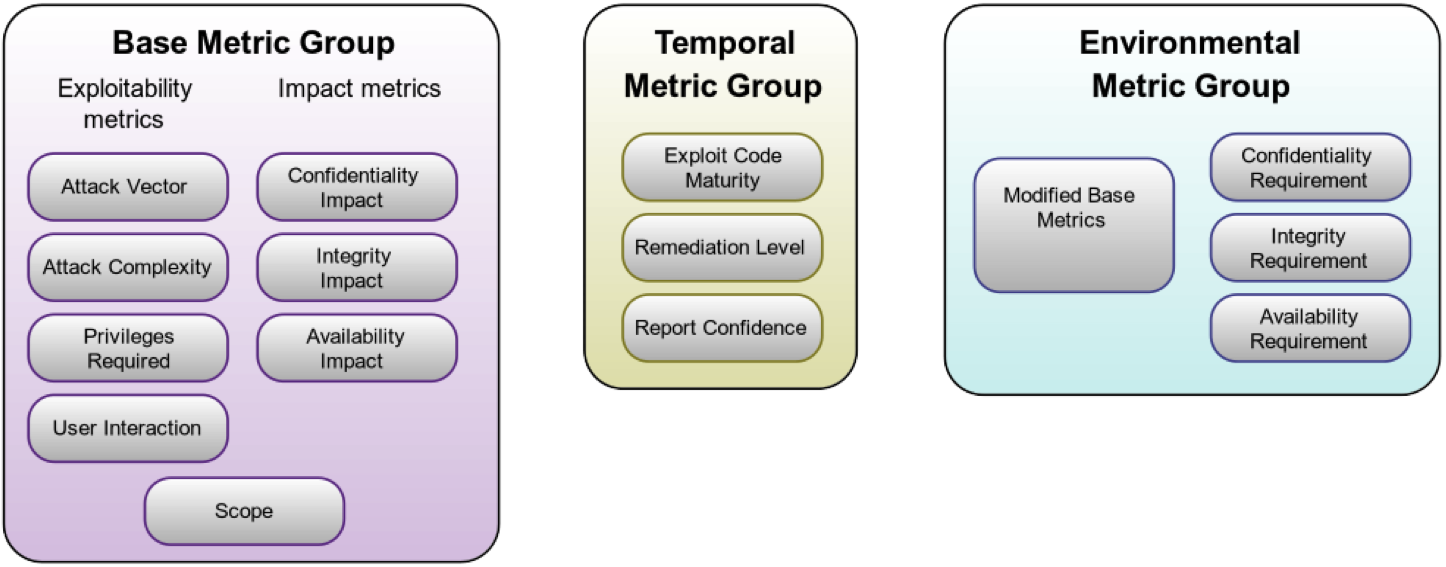
\includegraphics[width=0.9\textwidth]{obrazky-figures/cvss_metric_groups.png}
    \caption{Three CVSS metric groups. Source:~\cite{CVSSFirst}}
  \end{figure}

%   https://www.first.org/cvss/v3-1/cvss-v31-specification_r1.pdf
%   https://www.researchgate.net/publication/311694508_The_Common_Vulnerability_Scoring_System_CVSS_generations_-_usefulness_and_deficiencies

  \section{Vulnerability Databases}
  % https://wiww.researchgate.net/publication/316971384_Analyzing_Vulnerability_Databases
  In 1989 the Computer Emergency Response Team (CERT) was established at the Software Engineering Institute
  at Carnegie Mellon University to find, collect and publish all information about known vulnerabilities.
  After CERT displayed all collected vulnerabilities publicly, they started to appear in many new databases
  with different formats of weakness information. The most popular vulnerability databases were analysed
  in~\cite{VulnDBs}, but as of December 2022, some of them are shut down or not maintained.

  \subsection*{CVE -- Common Vulnerabilities and Exposures}
    CVE is a~list of publicly disclosed computer security flaws. It was released in 1999, at a~time when
    most cybersecurity tools used their own databases, names and evaluations of weaknesses. Now, CVE provides
    a~database and a~unified standard for naming information security vulnerabilities.

    The process of creating a~new CVE identifier begins with discovering and reporting a~potential security
    vulnerability. The information is accordingly assigned a~unique CVE identifier by a~CVE Naming Authority
    (CNA) and posted to the list on the CVE website by an editor. The MITRE Corporation functions as the editor
    and primary CNA~\cite{CVE}.

    Each entry in the list contains the following fields: CVE identifier number, brief description and references.
    The CVE identifier number format looks like ``\texttt{CVE--YYYY--NNNN}'', where
    ``\texttt{Y}'' refers to a~year of creation and ``\texttt{N}'' is unique number assigned to the vulnerability.
    As~of 29th December 2022, the database contains 191\,855 CVE records\footnote{\href{https://cve.mitre.org}
    {https://cve.mitre.org}} and is synchronized with the following database.

  \subsection*{NVD -- National Vulnerability Database}
  \label{section:nvd}
  The NVD was established in 2005 to provide the U. S. government with a~repository of data about software
  vulnerabilities. It is a~product of the National Institute of Standards and Technology (NIST) to provide
  vulnerability management information. The NVD can be used to prioritize the vulnerabilities to address
  in order to secure important systems.

  The database is based on and synchronized with the CVE list and enhances the base CVE scheme for vulnerability
  severity metrics and updates them when new information about the vulnerability is provided. CVSS is used
  for evaluation and helps to understand the potential severity of each vulnerability. NIST works directly
  with vendors and researchers to assure the quality of published information and provide the public with accurate
  scoring data~\cite{NVD}.

  Information about vulnerabilities is accessible to the public via the web page or REST API provided
  by the organization. As~of 29th December 2022, the database contains 203\,312
  records\footnote{\href{https://nvd.nist.gov/general/nvd-dashboard}{https://nvd.nist.gov/general/nvd-dashboard}}
  providing the following data:
  \begin{itemize}
      \item Base CVE Entry Schema -- Identification, Description, References
      \item Source Identifier -- Reporter
      \item Publication Time
      \item Last Modification Time
      \item Status
      \item Metrics -- CVSS
      \item Weaknesses -- contained CWEs
      \item Configurations -- CPE
  \end{itemize}

  \section{Real-world Example of Exploitation}
  The consequences of vulnerabilities in software applications can be quite serious like data breaches,
  theft of sensitive information, or damage to a~product infrastructure. For instance, consider
  vulnerability, in Microsoft Windows implementation of Server Message Block protocol, with an identifier
  CVE-2017-0144\footnote{\href{https://nvd.nist.gov/vuln/detail/CVE-2017-0144}{https://nvd.nist.gov/vuln/detail/CVE-2017-0144}}.
  An exploitation of this flaw, by sending crafted packets, allows remote attackers to run
  arbitrary code on a~target machine. This defect facilitated the spreading of worm-like ransomware
  \emph{WannaCry} through the network in 2017, which affected many organizations, companies,
  and individuals~\cite{WannaCry}. Figure~\ref{wannacryDistribution} depicts the spread of \emph{WannaCry} ransomware.
  % https://nvd.nist.gov/vuln/detail/CVE-2017-0144
  % https://www.zdnet.com/article/ransomware-an-executive-guide-to-one-of-the-biggest-menaces-on-the-web/

  Ransomware is a~type of malicious software, that locks up the victim's data or device and threatens to delete
  or keep it locked unless a~ransom is paid to an attacker~\cite{Malware}. In the case of \emph{WannaCry},
  the malware would encrypt files on the victim's device and ask for a~ransom of value 300 USD in Bitcoin
  if paid within the first three days, otherwise, the value would be doubled for the next four days and if
  not paid at all, the files would be lost forever.~\cite{wannacryBlog}
  % https://www.ibm.com/topics/ransomware
  % https://www.csoonline.com/article/3227906/wannacry-explained-a-perfect-ransomware-storm.html

  \begin{figure}[h]
    \centering
    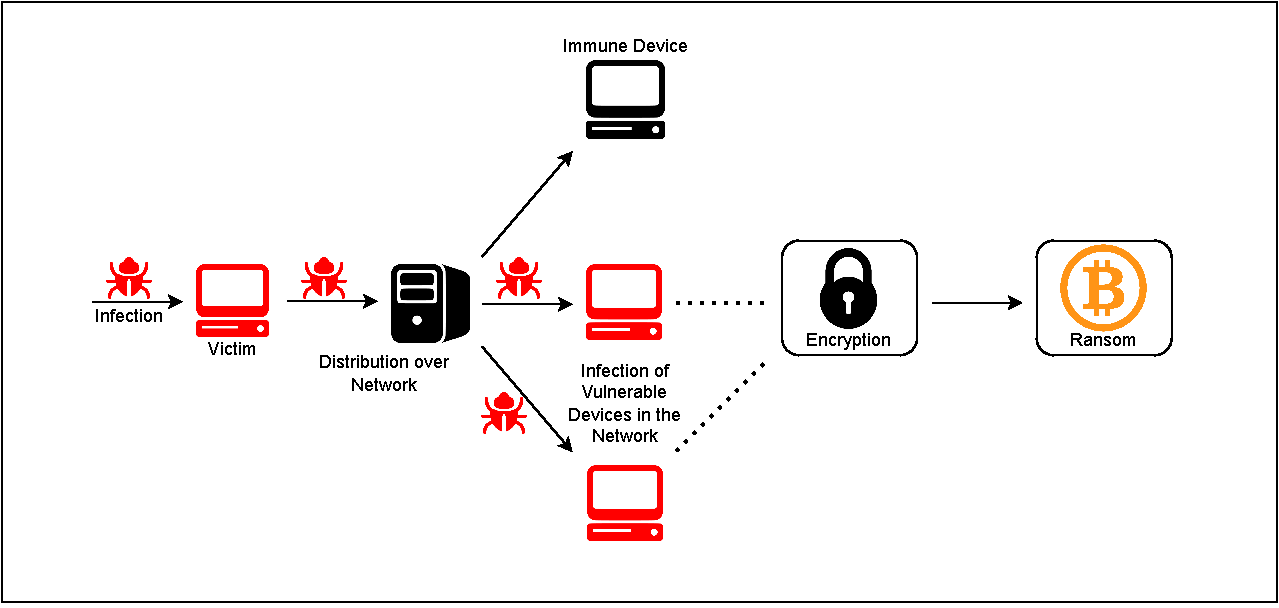
\includegraphics[width=0.9\textwidth]{obrazky-figures/wannacry_distribution_ransom.drawio.pdf}
    \caption{WannaCry ransomware distribution.}
    \label{wannacryDistribution}
  \end{figure}

    % File: src/chapter_3_clones.tex
% Project: Monitoring and Reporting Tool for Cloned Vulnerabilities across Open-Source Projects
% Author: Matus Remen (xremen01@stud.fit.vutbr.cz)
% Description: Chapter 3 - Cloned Vulnerabilities

\chapter{Cloned Vulnerabilities}
\label{chapter:clonedVulnerabilities}
Cloned vulnerabilities are weaknesses propagated by reusing source code. This can happen by copy-pasting
insecure code snippets, whole functions or even whole projects. For copying the whole project version control system
Git offers an easy option called a~fork. This allows developers to inherit the infrastructure of an existing project
and afterwards they can modify or start building on it their own features. Although, the inherited code base might
contain vulnerabilities.

In the beginning, this chapter will present an example of a~vulnerability propagated by cloning, followed by
an overview of clone types based on the level of similarity to the origin and methods for their detection. Afterwards,
existing static analysis tools and approaches for the detection of cloned vulnerabilities in the software
will be analysed.

\section{Real-World Example of a~Cloned Vulnerability}
\label{sec:example-cloned-vuln}
  A~notable case of a~flaw propagated by forking or fetching is CVE-2018-17144. On the 18th of September 2018, the bug
  was patched in Bitcoin Core, the primary implementation of the Bitcoin protocol. Besides a~potential Denial of Service (DOS)
  attack, the vulnerability allowed an attacker to double-spend the same input, which would create new bitcoins out of nothing
  and cause inflation in this major cryptocurrency. The flaw was caused by an unhandled assertion error in a~code validating
  transactions and preventing double spending of coins.~\cite{BTCInflationBug, HackerNoonBTCInflationBug}

  \begin{figure}[h]
    \centering
    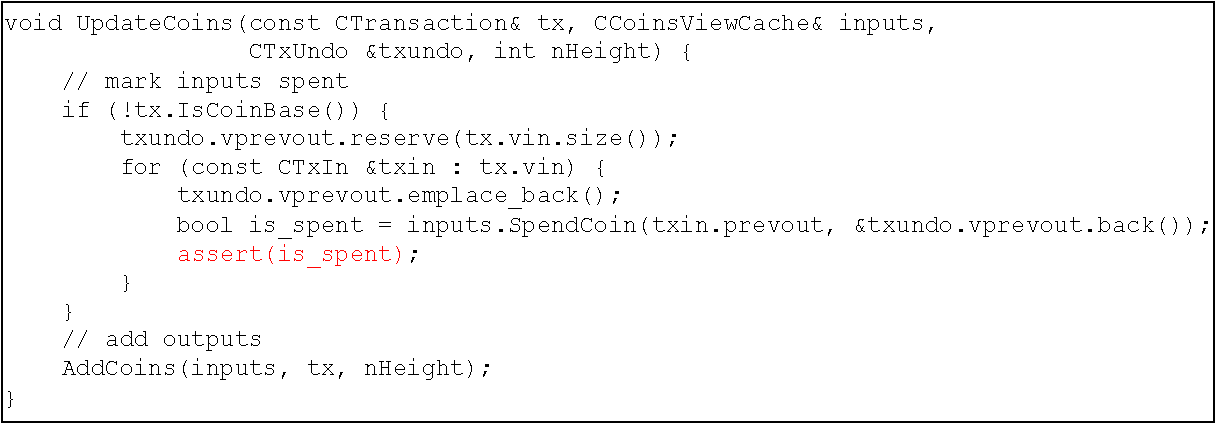
\includegraphics[width=0.9\textwidth]{obrazky-figures/cve-2018-17144_code.drawio.pdf}
    \caption{Vulnerable code shared between Bitcoin and PigeonCoin. Source:~\cite{BTCInflationBug}}
    \label{cve201817144code}
  \end{figure}

  The bug was fixed in Bitcoin Core before it could have been exploited. Unfortunately, in the case of PigeonCoin,
  one of many forks of Bitcoin, attackers took advantage and generated 235~million coins worth of around 15,000 USD
  on 26th of September 2018, while it was still vulnerable more than a~week after the fix in Bitcoin Core.
  The propagated code responsible for the vulnerability is visible in Figure~\ref{cve201817144code}.~\cite{CoinDeskPGNInflationBug,
  HackerNoonBTCInflationBug}
  % TODO 2 more

\section{Types of Code Clones}
  Clones of source code originate from copying and reusing code fragments with possible modification
  is a~common approach in software development. Such activity is an efficient way in programming as similar
  code does not have to be written multiple times from scratch. Depending on how similar the code clones are to
  their origins, they are divided into four groups~\cite{CodeClonesSurvey}. For an example of each type of clone
  consider the following code in the programming language C as the original code:
  \begin{alltt}
  if (a > b) \{  // comment
      a = b + 1;
  \} else \{
      a = b + c;
  \}
  \end{alltt}
  \textbf{Type~I} clones are identical code fragments with possible white space characters and comment
  variations.
  Type~I clone from the example original code could be:
  \begin{alltt}
  if (a > b) \{
      a = b + 1; \textcolor{red}{\}  // comment 1}
  else \{
      a = b + c; \textcolor{red}{\}  // comment 2}
  \end{alltt}
  \textbf{Type~II} are Type~I clones with additional possible variations in user-defined identifier naming
  and types. An example could be:
  \begin{alltt}
  if (\textcolor{red}{x} > \textcolor{red}{y}) \{
      \textcolor{red}{x} = \textcolor{red}{y} + 1;  \textcolor{red}{// comment}
  \}
  else \{ \textcolor{red}{x} = \textcolor{red}{y} + \textcolor{red}{z}; \textcolor{red}{\}}
  \end{alltt}
  \textbf{Type~III} clones in addition to Type~I and Type~II contain changed, added and/or deleted statements.
  Type~III clone might look like this:
  \begin{alltt}
  if (x > y) \{
      x = y + 1;
  \} else \{  // comment
      \textcolor{red}{flag = 1;  // addition}
      x = y + z;
  \}
  \end{alltt}
  \textbf{Type~IV} are code fragments with different syntactical structures, but with the same semantics. Unlike
  the previous types which were textually similar, this type of clone is defined by functional similarity.
  An example of a~Type~IV clone might look accordingly:
  \begin{verbatim}
  x = x > y ? y + 1 : y + z;
  \end{verbatim}

\section{Detection Methods}
  Detection techniques are divided into four classes: textual, lexical, syntactic and semantical.
  This section will introduce each class and mention detection tools which are based on them.

  \subsubsection*{Textual Approaches}\label{clone-detection:simian}
    Text-based approaches compare two code fragments and detect clones based on string comparison of lines.
    They are language-independent, easy to implement and generate fewer false positive results. Before detection,
    they tend to use normalization like the removal of white spaces and comments. This approach is able to detect
    Type~I clones without further post processing~\cite{CloneDetectionTechniques, CodeClonesSurvey}. Tools which
    are based on this approach include Dup~\cite{Dup} and NICAD~\cite{NICAD}.

  \subsubsection*{Lexical Approaches}
    In lexical or token-based approaches whole source code of the analysed project(s) is parsed into a~sequence
    of tokens. Then in the next step, the generated sequence of tokens is scanned for duplicate subsequences which
    represent code clones in the end. CCFinder~\cite{CCFinder} and CPMiner~\cite{CPMiner} are example tools
    utilizing this approach. They are able to detect clones of various types and have higher precision than
    textual approaches, but they also have some limitations. These techniques have higher time and space
    complexity and are dependent on the order of the tokens and lines. When cloned code contains added or deleted
    tokens, this approach will not detect it as clone~\cite{CloneDetectionTechniques, CodeClonesSurvey}.

  \subsubsection*{Syntactic Approaches}
    Syntactic approaches contain two types of techniques -- tree-based and metric-based.

    Tree-based approach parses the source code of the analysed project firstly into tokens which are used
    to build an abstract syntax tree (AST). Then the clones are detected using tree-matching algorithms rather
    than matching sequences of tokens in lines as in lexical approaches. In this case, similar sub-trees
    represent duplicate code. Tools developed by Baxter et al.~\cite{ASTBaxter} and by Wahler et
    al.~\cite{ASTWahler} implement the tree-based approach.

    The second type, the metric-based approach uses a~number of different metrics gathered from syntactic units
    like classes, methods, functions or statements in the target source code. The metric vectors are then compared
    in order to detect clones instead of searching through AST or comparing code directly. Some of the collected
    metrics in tools implementing this approach can be numbers of loop, conditional and return
    statements~\cite{CloneDetectionTechniques, CodeClonesSurvey}.
    Implementations of metric-based approach are for example tools developed by Mayrand et al.~\cite{MBMayrand}
    or by Abdul-El-Hafiz et al.~\cite{MDAbdul}.

  \subsubsection*{Semantic Approaches}
    This type of approach is used to detect code fragments with similar semantics but different code structures.
    There are two approaches connected with this technique -- graph-based and hybrid.

    The graph-based approach utilizes a~Program Dependency Graph (PDG) to represent data and control
    the flow of the analysed source code. The detection is performed by an isomorphic subgraph matching algorithm.
    For example, tool GPLAG~\cite{GPLAG} implements this approach.

    The hybrid detection technique combines multiple approaches which were mentioned
    above~\cite{CloneDetectionTechniques, CodeClonesSurvey}. An approach developed by Agrawal et
    al.~\cite{HybridAgrawal} uses this technique.

\section{Detection Tools}
Detection tools and approaches analysed in this section are tools designed for the automatic identification of
security vulnerabilities in software applications. Common types are static analysis tools,
dynamic analysis tools and penetration testing tools. Static analysis tools scan software source code
to identify potential weaknesses, while dynamic analysis tools observe the behaviour of the system during
run-time. Penetration testing tools are designed to simulate attacks on the system to identify
vulnerabilities, which might be exploited during a~cyberattack.

  \subsection*{CoinWatch}
    \textit{This subsection is based on~\cite{CoinWatch}.}
    CoinWatch is a~static analysis tool utilizing a~clone-based approach for detecting vulnerabilities
    in cryptocurrencies. Cryptocurrencies are an attractive commodity for attackers because they can be
    anonymously sold on exchanges. The fact, that many of them have their source code publicly available,
    makes it possible to develop tools like CoinWatch. It was developed in 2020 and has achieved promising
    results, but unfortunately, it is not available for public use.

    In summary, CoinWatch reported 786 vulnerabilities in 384 cryptocurrencies to the date, when the paper
    was written and achieved a~true positive rate of 89.7\%. To the date, CoinWatch worked only with Type~I
    clones, while Type~II and Type~III would need a~more sophisticated method of detection like analysis of
    decompiled binaries of projects. In future work, creators want to investigate possibilities for how to
    detect also Type~II and Type~III clones alongside automating the process of the manual code
    annotation.

    A~study connected with CoinWatch contains an analysis of the propagation of cloned source code between
    cryptocurrencies. The analysis found that at the time 786 cryptocurrencies were directly or indirectly
    cloned from a~version of Bitcoin. The percentage of cloned code in projects forked from Bitcoin
    is displayed in Figure \ref{bitcoin-clone-ratio}. In the majority of these projects, the clone ratio was
    below 30\%, however, some had the ratio even higher than 50\%. This fact implies the potential propagation
    of vulnerabilities among clones, once they are discovered in the parent project. In the case of
    cryptocurrencies, neglecting the maintenance of the adopted code may have a~serious financial impact.
    Also, the number of detected projects by the analysis is high, which makes maintenance a~very costly
    and repetitive task. CoinWatch is a solution for filtering only potentially vulnerable projects,
    whose maintainers can be accordingly warned about the detected threat.

    \begin{figure}[h]
      \centering
      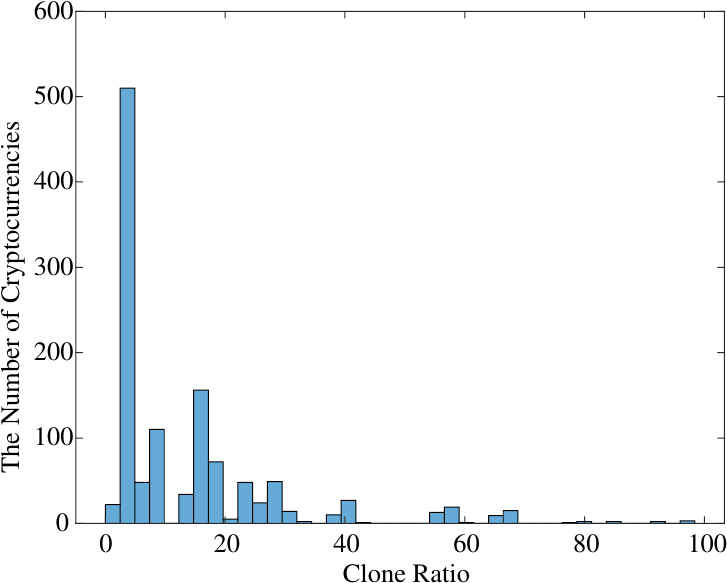
\includegraphics[width=0.5\textwidth]{obrazky-figures/clone_ratio_histogram.png}
      \caption{Bitcoin v0.17.0 clone ratio in forked projects. Source:~\cite{CoinWatch}}
      \label{bitcoin-clone-ratio}
    \end{figure}

    The overall workflow of CoinWatch is visualized in Figure~\ref{coinwatch-workflow}. At the beginning
    of the pipeline, the tool receives a~target CVE assigned to the target project. Accordingly, all publicly
    available details about the desired vulnerability are scraped and parsed from vulnerability databases.
    These details are input for the next step -- code evolution analysis. The analysis utilizes the version
    control system Git for traversing the versions of the target project. Using the parsed CVE details,
    the analysis aims to identify fixing and bug-introducing commits for the provided vulnerability
    in the repository of the project. Identified fixing and bug-introducing commits create a~time window, in which
    the target project was affected by the vulnerability. This time window is used for the initial filtering
    of potentially affected child projects, which were forked from the target project during this period.
    The identified fixing and bug-introducing commits are additionally used for manual annotation of
    the vulnerable code and transformation to a~clone detection pattern. In the end, the clone detection tool
    checks the occurrence of the pattern in the potentially vulnerable projects forked in the time window.
    After clone detection, on the output of the pipeline is a~list of likely affected cryptocurrencies.

    \begin{figure}[h]
      \centering
      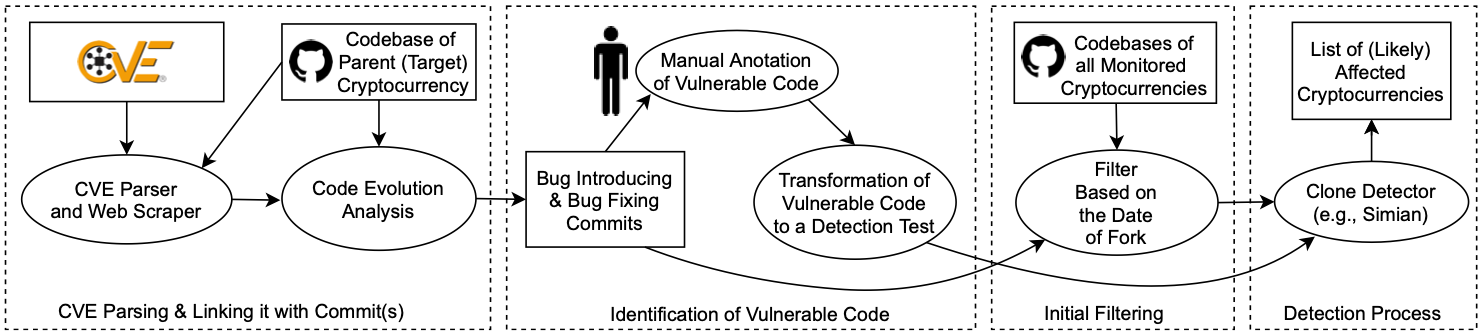
\includegraphics[width=1\textwidth]{obrazky-figures/coinwatch_workflow.png}
      \caption{Overall workflow of tool CoinWatch. Source:~\cite{CoinWatch}}
      \label{coinwatch-workflow}
    \end{figure}

    \subsubsection*{CVE Parsing and Linking with Commits}
      In this step, CoinWatch scrapes and parses details of the selected vulnerability. Following data
      is extracted from details about CVE in vulnerability databases:
      \begin{itemize}
          \item date of publishing
          \item keywords from description
          \item references pointing to the version control system of the affected project
          \item the list of affected cryptocurrencies and their programming language
      \end{itemize}
      After parsing, the origin of the vulnerability is checked, and whether the issue is connected with specific
      code as the threat may originate from using outdated versions of libraries, frameworks and protocols.
      In case of code-specific weakness, the code evolution analysis links patching and bug-introducing
      commits with the CVE.

    \subsubsection*{Code Evolution Analysis -- SZZ Algorithm}
    For the purpose of code evolution analysis, CoinWatch utilizes the SZZ algorithm. The algorithm was proposed
    by Sliwerski, Zimmermann and Zeller~\cite{SZZalgorithm} as an approach for identifying bug-introducing
    commits. An open implementation of the algorithm is named SZZ Unleashed~\cite{SZZunleashed}. It is written
    in Java programming language with supporting Python scripts. SZZ Unleashed works in two phases. The first
    phase identifies bug-fixing commits used in the second phase for tracking the bug-introducing changes.
    CoinWatch is built on this algorithm and extended it for the tool's specific purposes.

    Firstly, using parsed details about the vulnerability, the bug-fixing commits are identified from
    the version control system in the affected project. In CoinWatch this is done by matching regular expressions
    in issues which have been fixed, resolved, closed or labelled as ``bug''. The regular expression is built
    from keywords extracted from the description in CVE details and keywords ``CVE'' and ``CVE-ID''.

    Secondly, for each discovered fixing commit the bug-introducing commits are tracked utilizing the second
    phase of the SZZ algorithm. This phase leverages the command git-blame and line number mapping to backtrack
    through the history of the analysed project. This method maps only the lines affected by the
    analysed commit as shown in Figure \ref{szz-line-map}. In addition, this phase provides an option to
    select the desired depth of mapping the line numbers over a~variable number of versions, indicated by
    the depth parameter. In the provided example, working with the depth option set to one would result in
    not identifying the bug introduced by Commit 2, because it is in depth two and it is detectable only from
    the annotation of commits 3, 4 and 5.

    \subsubsection*{Identification of Vulnerable Code and Initial Filtering}
    Inputs for this part of the CoinWatch are bug-fixing and their matching bug-introducing commits.
    For initial filtering of potentially vulnerable forks, CoinWatch selects the newest bug-fixing commit
    and the oldest bug-introducing commit to form a~time window. Monitored forked projects are then filtered
    based on the timestamp of their fork. When it is within the time window they are marked as potentially
    vulnerable candidates. The projects around the time window are ignored.

    Identification of vulnerable code is a~one-time manual process per CVE. The goal of this step is to
    extract the patch code and the vulnerable code from commits detected during code evolution analysis.
    After the manual code annotation, it is transformed into a~detection test as input for the clone detection
    tool.

    \begin{figure}[h]
      \centering
      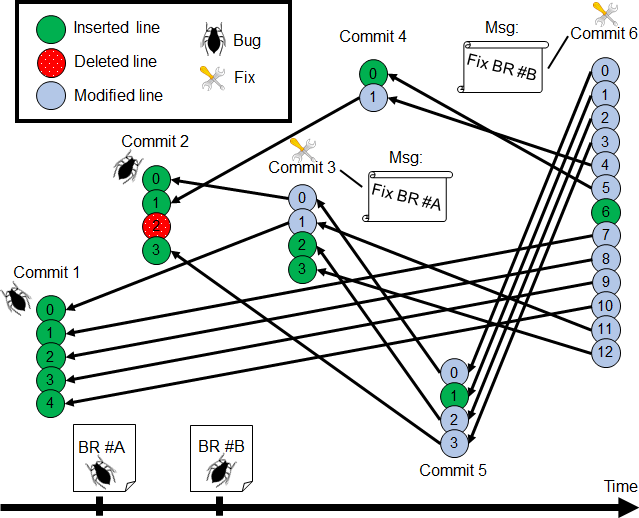
\includegraphics[width=0.7\textwidth]{obrazky-figures/szz_line_mapping.png}
      \caption{An example of SZZ Unleashed mapping line numbers. Source:~\cite{SZZunleashed}}
      \label{szz-line-map}
    \end{figure}

    \subsubsection*{Clone Detection Process}
    Finally, CoinWatch triggers the clone detection tool Simian \ref{clone-detection:simian} with the detection
    test on the list of potentially vulnerable candidates from the previous step. This filters the projects
    that already patched the vulnerability or reimplemented the part of code, which was vulnerable in the
    source project and returns the final list of likely vulnerable projects.

  \subsection*{BlockScope}
  \label{section:blockscope}
    \textit{This subsection is based on~\cite{BlockScope}.}
    BlockScope is a~novel tool for detecting vulnerabilities propagated by cloning blockchain projects like
    Bitcoin and Ethereum. It is a~language-agnostic tool capable of detecting multiple vulnerabilities from
    existing security patches. BlockScope utilizes similarity-based code match and designs
    a~new way of calculating code similarity. Thanks to this approach it is able to detect Type~I, Type~II and
    Type~III clones. Additionally, it is capable of automatic extraction of security patch contexts in comparison
    to CoinWatch.

    Figure \ref{blockscopeworkflow} presents the overall workflow of BlockScope. Initially,
    the tool receives a~security patch and the affected project on the input. The security patch is accepted
    either in the form of a~commit ID from the source project or manually crafted patch contexts for better accuracy.
    A~patch context represents a~surrounding of the code changes in the patch commit. The component named
    Extractor serves for identifying patch context when the commit ID of the security patch is provided.
    Subsequently, the component Searcher tries to match the patch context in the analysed project which produces
    a~candidate context. Then Fetcher uses the contexts to extract patch code from the source project
    and potentially vulnerable candidate code from the target project. The similarity of the extracted
    codes is then measured in Comparator, which determines whether the target project was patched. Additionally,
    for the vulnerabilities that were already fixed in the target repository, BlockScope performs
    the calculation of patch delay.
    \bigskip
    \begin{figure}[h]
      \centering
      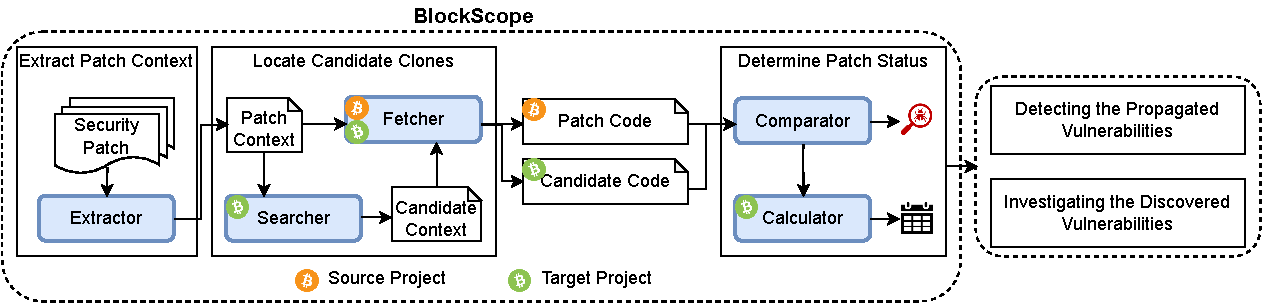
\includegraphics[width=0.99\textwidth]{obrazky-figures/blockscope_workflow.pdf}
      \caption{Overall workflow of tool BlockScope. Source:~\cite{BlockScope}}
      \label{blockscopeworkflow}
    \end{figure}

    BlockScope achieved overall precision and recall both at the rate of 91.8\%. It discovered 101 previously
    unknown vulnerabilities propagated via code cloning in 13 out of 16 analysed projects forked from Bitcoin
    and Ethereum. Unfortunately, just like CoinWatch it is not available for public use and is
    close sourced.

    \subsubsection*{Patch Context Extraction}
    The initial step of BlockScope extracts the context of the given security patch on the input. The patch context
    consists of two components -- upper and lower. The extraction is depicted in Figure~\ref{figure:blockscope-search}
    on a~patch code on the left side and the process is following.

    Firstly, the code surrounding the patch is tokenized. Tokenization considers both upper and lower case characters
    and additionally includes some special characters such as ``.'' and~``!''. Then, in each context line, the longest
    token is selected as a~keyword representing the sentence. The keywords together identify the patch context in the next
    step in the processing. In the example displayed in Figure~\ref{figure:blockscope-search}, the selected keywords
    are marked by a~red font colour.

    \subsubsection*{Localization of Candidate Code Clones}
    In this step, BlockScope searches for all candidate code clones in target repositories using components Searcher and Fetcher.
    Figure~\ref{figure:blockscope-search} illustrates this process on patch commit \texttt{0e7c52dc} in Bitcoin
    and a~cloned code chunk present in Dogecoin, a~fork of Bitcoin.

    The localization begins with selecting key statements from each patch context in the target repository.
    To determine key statements, the component Searcher firstly utilizes a~command \texttt{git grep} to find
    all code statements containing the patch keywords extracted in the previous step. Finally,
    each found code statement is compared to the original code statement in the patch context and the most similar
    one is selected as a~key statement in each context.
    For calculating the similarity, BlockScope uses the Normalized Levenshtein edit distance metric with a~threshold
    equal to 0.25.

    The threshold is used to minimize misses and avoid false negative results in the rest of the workflow.
    In the current step, the threshold is used to filter code statements with low similarity to the original
    statement. Additionally, the tool uses here three other optimizations. The first excludes comments and test code
    from keyword search results. The second filters search results based on the type of file affected by a~patch
    and the third checks the type of code statements.

    Once the key statements are identified, the goal of the next step is to extend the single statement to multi-line
    candidate context. This is done by extracting the surrounding code around the key statement until the candidate
    context contains the same number of lines as the patch context, which is specified by a~constant \texttt{C\_LINES}.
    Then, the boundary is determined by comparing each line in the candidate context to the start and end statements.
    In the end, just like in the case of the key statement, the start and end statements in the candidate context are specified
    by the highest similarity exceeding the threshold.

    Finally, the candidate contexts are yet compared to the patch using the same evaluation method as used for
    determination of patch application status~\ref{similarity-equation}.
    Candidate contexts with similarity below the threshold are discarded and the others are forwarded to the component
    Fetcher. As for the patch, so for candidate contexts, the component Fetcher extracts the code between the upper and lower
    context, returning a~patch code and a~list of candidate codes for further analysis.

    \begin{figure}[h]
      \centering
      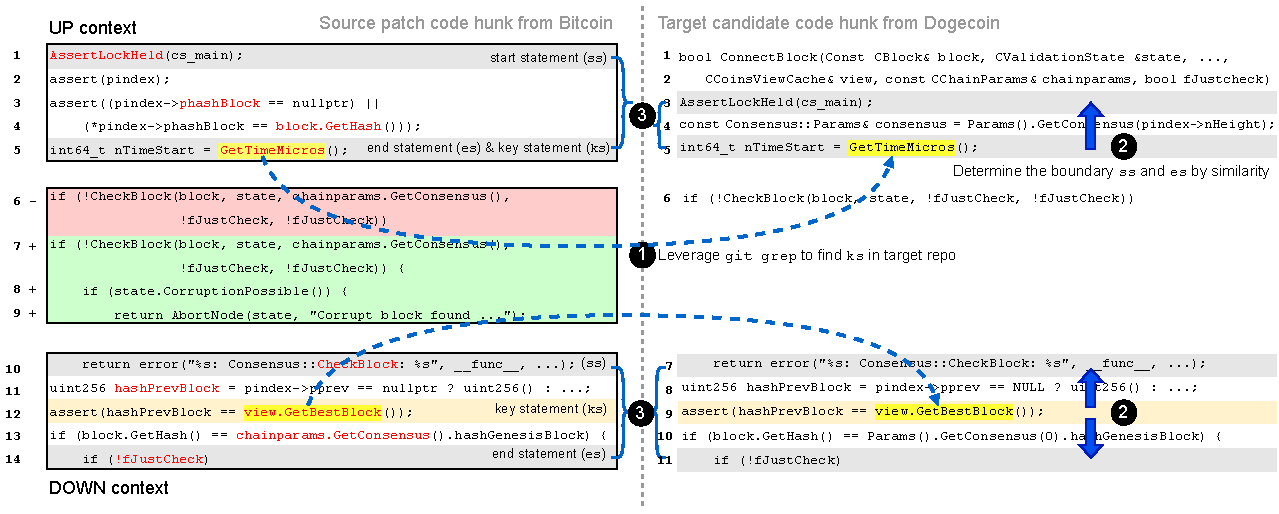
\includegraphics[width=1\textwidth]{obrazky-figures/blockscope_search.drawio.pdf}
      \caption{Visualization of context-based search of BlockScope for searching candidate contexts in a~target repository.
       Source:~\cite{BlockScope}}
      \label{figure:blockscope-search}
    \end{figure}

    \subsubsection*{Determination of Patch Status}
    The last step of the workflow, the determination of the patch application status is performed in components Comparator
    and Calculator. The Comparator measures the similarity between the patch and each candidate and evaluates, whether
    the target project applied the patch, hence whether it is vulnerable or did not inherit that particular part
    of the code. The projects, which applied the patch are further analysed by the component Calculator, which
    calculates a~patch delay.

    BlockScope designs a~new way of measuring the similarity between two code fragments, which is capable of detecting
    the first three types of clones. The way is shown in the following Equation~\ref{similarity-equation}, where
    $S$ stands for source and $T$ for target code fragment with $p$ and $q$ code statements. The similarity measure
    is defined as the weighted average of the similarity of each sentence from $S$ and its most similar pair among $T$.
    The function $strsim$ calculates the Normalized Levenshtein distance metric~\cite{strsim} of two strings, which returns a~value
    in the interval $[0, 1]$. To cover clones of Type~III, as they contain inserted, deleted and reordered statements,
    this way introduces parameter $r \in [0, 1]$ and $r^{\vert i-j \vert}$ to specify the reward of the similarity result
    between $S_i$ and $T_j$.

    \begin{equation}
      \begin{aligned}
        \text{SIMILARITY}(S, T)\ &=& \frac{1}{p} \sum \limits^p_{i=1}\text{strsim}(S_i, T_j)r^{\vert i-j \vert} \\
        \text{s.t. } j\ &=& \mathop{arg\ max\ }_{1 \leq k \leq q} \text{strsim}(S_i, T_k)
        \label{similarity-equation}
      \end{aligned}
    \end{equation}

    To determine whether a~patch ($P$) was applied, it is compared to the candidate code ($C$) and BlockScope uses three
    rules for that evaluation. There are three possible types of patches. One which contains only code additions (\texttt{ADD} type,
    $P = [ap]$), a~one with code deletions only (\texttt{DEL} type, $P = [dp]$) and the third, which contains both
    (\texttt{CHA} type, $P = [ap, dp]$). Using the described similarity measure, each type has its own definition of applied status.
    Consider variables $sa = SIMILARITY(C, ap)$ and $sd = SIMILARITY(C, dp)$ for better readability in the following description
    of the rules for each type.
    \begin{itemize}
        \item \texttt{ADD} type: if $sa \geq t$, it is evaluated, that $P$ was applied in $C$, else it was not.
        \item \texttt{DEL} type: if $sd \geq t$, it is evaluated, that $P$ was not applied in $C$, else it was.
        \item \texttt{CHA} type: if $sd \geq t$ and $sa \geq t$ and $sd \geq sa$, it is evaluated that $C$ did not apply $P$,
              otherwise if $sd \geq t$ and $sa \geq t$ and $sd < sa$, it is evaluated that $C$ applied $P$
    \end{itemize}

    The components from the previous step can return more than one candidate context, and so produce multiple candidate
    code fragments $C_i \in [C_1, C_2, ..., C_n]$. In this case, similarity of each candidate, $s_i = SIMILARITY(C_i, P)$,
    and its patch application status, $fv_i \in \{0, 1\}$, is calculated, where $f_i = 1$ indicated, that $C_i$ applied patch $P$.
    To finalize the results, factor $conf_i = s_i - t$ is introduced to measure the confidence of each result. In the end,
    the result with highest confidence $fv_i$, where $i = arg\ max_j\ conf_j$, is selected as the final result of application
    status.

    Projects, which already applied the patch are additionally analysed by component Calculator. Calculator leverages
    command \texttt{git blame} to extract the hash of the commit, which patched the vulnerability in the target repository.
    The command returns additionally to each line of code in the provided file the latest commit, which changed the line.
    Using this information, the commits on the lines of candidate code are fetched. If the candidate code was changed
    by multiple commits, the earliest one is considered as fixing. In the end, the component Calculator calculates
    the delay between the patch commit in the original repository and the extracted commit in the target repository.

% https://www.researchgate.net/publication/335152710_Detecting_Security_Vulnerabilities_using_Clone_Detection_and_Community_Knowledge

    % File: src/chapter_4_design.tex
% Project: Monitoring and Reporting Tool for Cloned Vulnerabilities across Open-Source Projects
% Author: Matus Remen (xremen01@stud.fit.vutbr.cz)
% Description: Chapter 4 - Design

\chapter{Design}
\label{chapter:design}
  This chapter presents the design of the proposed tool which, aims to address the challenges and requirements
  identified in the problem of detecting cloned vulnerabilities. It is organized into three main sections, each focusing
  on a~key aspect of the tool: architecture, workflow and user interface. These sections provide an overview
  of how the monitoring tool is structured, how it works, and how to interact with it.

  \section{Architecture}
  \label{section:architecture}
    In this section, the structural design of the tool is displayed. Presenting a~clear and organized
    view of its architecture, this section aims to demonstrate how various elements in the system work
    together to form a~coherent whole.

    Figure \ref{architecture} depicts the parts of this tool and the communication between them.
    The core of the application consists of the detection mechanism and its internal database. To interact
    with the core, it has available a~command line interface and a~web interface. The command line interface
    has direct access to the core of the tool, while the web is connected to the core via the application
    programming interface. All together builds a~tool offering two modes for detecting cloned vulnerabilities.
    The first one detects the propagation of a~specific vulnerability among the clones of the project where it was discovered.
    The second method discovers new flaws but is executable only from the command line.

    \bigskip

    \begin{figure}[h]
      \centering
      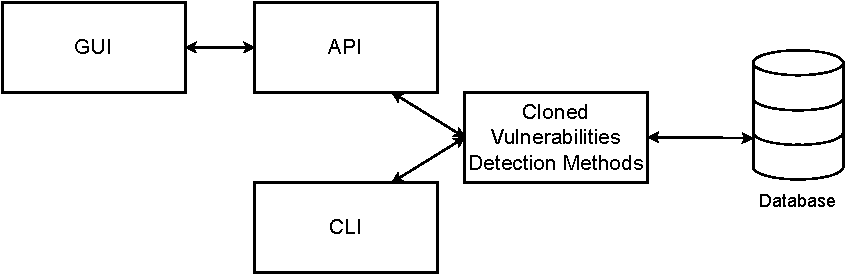
\includegraphics[width=0.95\textwidth]{obrazky-figures/architecture.drawio.pdf}
      \caption{Architecture of the tool.}
      \label{architecture}
    \end{figure}

    \subsection*{Database Schema of the Tool}
    \label{design:database}
    The database consists of two primary and one secondary entity set represented by an entity relation diagram
    in Figure~\ref{erd}. The primary entities contain configurations supporting the automation rate and scope
    of the detection mechanism. The secondary entity is used as a~container for vulnerability detection
    results and has no effect on the performance of the tool.

    The entity \texttt{Bug} contains details about vulnerabilities like an identifier in case of CVE, a~commit
    responsible for the repair of the bug, a~patch containing specific fix changes and a~code for particular
    methods for detecting clones. Depending on the configured method, if available, the patch is used
    by integration of BlockScope described in Section~\ref{section:blockscope}. While the value in attribute \texttt{code}
    would be used by an integrated clone detection tool Simian\footnote{\href{https://devel.nuclex.org/external/svn/simian/trunk/index.html}
    {https://devel.nuclex.org/external/svn/simian/trunk/index.html}}.
    Additionally, this entity contains attribute \texttt{verified} to inform about whether the bug was reviewed
    by an administrator as all records in this table are created automatically during the run of the detection
    method. Firstly, in the case of CVE records, the vulnerability databases do not always refer explicitly
    to the specific fix commit or patch, but it is detected by various scans which will be mentioned in the next
    Section \ref{section:workflow}. Secondly, the application programming interface (API) of the National Vulnerability
    Database~\ref{section:nvd} has a~limited availability of five queries per rolling thirty seconds time window\footnote{
    \href{https://nvd.nist.gov/developers/start-here}{https://nvd.nist.gov/developers/start-here} -- rate limits}.
    Storing and reusing previously requested data prevents from reaching the query limit and allows to subsequently
    further edit and specify particular details, so the tool can process them faster and run smoother.
    Lastly, the attribute \texttt{created} contains a~timestamp of record creation, which represents scan times.
    The repositories can be updated over time and older scans might not be relevant since new commits were released
    and the identified bugs could be fixed. The relation \texttt{discovered in} binds a~bug to the project where it was found.
    Overall, the~attributes of this entity support the performance of the tool and allow it to run automatically
    skipping the~step of the manual selection of the relevant patch code.

    On the other hand, the entity set \texttt{Project} not only offers performance benefits but also contains important
    data related to the configuration of the workflows. The attribute \texttt{url} contains a~link used for initialization
    of the repositories by cloning to a~fresh environment of the tool, after adding a~new project or basically
    when it is missing. Attribute \texttt{name} and~\texttt{author} are used mainly for easier referencing from user input
    and logs. The \texttt{language} contains the programming language of the project for filtering the relevant
    files and code in the repository. The value of attribute \texttt{watch} marks projects which are updated and checked
    daily for potential vulnerability patching commits. Lastly, the timestamp in the attribute \texttt{added}, informs
    about the time of registration. The relation \texttt{forked by} models the~hierarchy of parent and cloned projects
    which are used in the detection methods to~decide which projects are potentially affected by a~cloned vulnerability.
    Accordingly, the detection is performed only among them. The records in this table are created on demand during
    the process of project registration.

    Lastly, the entity set \texttt{Detection} represents only positive results of detection methods which form a~relation
    between bugs and forked projects. Additionally, it also provides confidence in the result and the timestamp.
    Confidence is a number in the range of 0.0 -- 2.0, which represents the similarity of patch code and target code.
    Information from these entities does not affect the tool but serves as a~storage of results from previous scans.
    Consequently, the results can be cross-checked, and the maintainers of~affected projects can be notified about the presence
    of the cloned vulnerability.

    \begin{figure}[h]
      \centering
      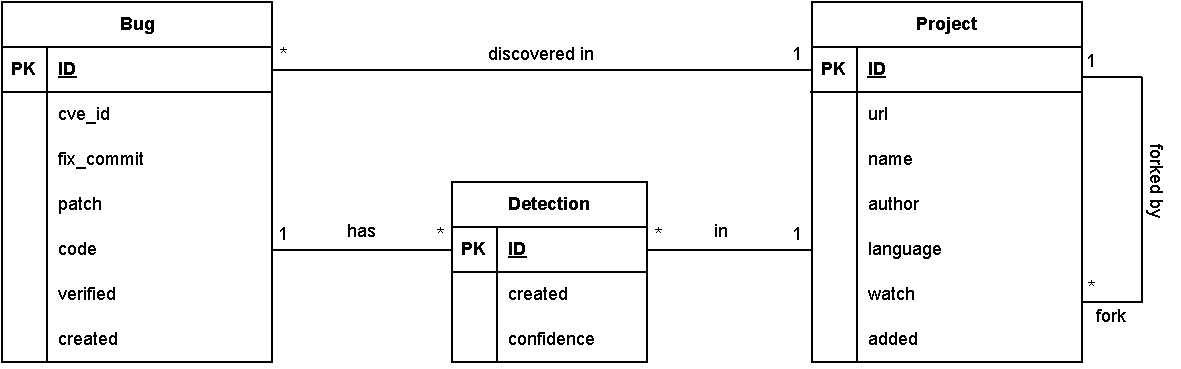
\includegraphics[width=0.95\textwidth]{obrazky-figures/cloneguard_erd.drawio.pdf}
      \caption{Entity relation diagram.}
      \label{erd}
    \end{figure}
    \bigskip

  \section{Workflow of the Detection Mechanisms}
  \label{section:workflow}
  As already mentioned in the previous section, the tool has two modes for detecting cloned vulnerabilities.
  The process of the first mode is similar to the CoinWatch and BlockScope. The second one
  performs periodic scans of parent repositories with an attempt to detect new potential
  flaws from recent patch commits. This functionality extends the detection options of the mentioned tools.

  \subsection*{Targeted Detection}
  \label{section:targeted-detection}
  The workflow of the targeted detection is displayed in~the~Figure~\ref{cg-workflow1}.
  It is executed on demand and requires an input, which contains a~reference to~vulnerability and the name of the project
  where it was discovered. It is mandatory for the project to be registered in the database prior to the vulnerability detection scan, so the mechanism
  has available all the required information about it.

  If the requirements are met, the detection mechanism starts with collecting information about the provided weakness
  and~initializes the repository of the target project. Firstly, the tool checks whether the provided reference
  to the vulnerability is available in the internal database. Otherwise, if CVE ID was provided the tool fetches
  its data using a vulnerability identifier from NVD using their API and stores the response in a~cache. Consequentially,
  based on the fetched
  data the patch commit is searched in the target repository. Afterwards, if it was not in the internal database
  before, it is stored here. If the search found multiple candidate commits or one is very extensive, the user
  is requested to specify the patch commit and code that is responsible for fixing the~vulnerability to reduce the number
  of candidates. This input is accordingly stored in the created record in the database.

  In the next step, all registered forks of the target project are initialized. That means if~their repositories
  are missing in the local storage of the tool, they will be cloned using attribute \texttt{url} of entity \texttt{Project}.
  In case they are downloaded, they are updated by pulling changes from their remote repository.
  It is also possible to~configure the tool to downgrade the repositories to an older version, which will be utilized
  in experimentation with the tool.
  This can be achieved by providing a~specific date in the input of the tool. In that case, the last commit
  before the~provided date will be selected and the repository will be reverted to that particular commit.

  At this point, all potentially affected projects are prepared for further investigation of~possible
  propagation of the vulnerability during forking or preliminary fetching. In the default setup, a~detection
  method based on the approach presented in the research paper about BlockScope is used~\cite{BlockScope}. Firstly,
  the surrounding code chunks -- contexts are fetched from fixing commit or directly from specific patch code
  present in attribute \texttt{patch} in the database. The~patch contexts are then searched for in the prepared
  set of repositories based on the code similarity. The detected contexts and the code in between then produce
  candidate code chunks, which are in the end compared to the patch code. In the end, based on the similarity
  of the patch and candidate code, the tool determines whether the patch was applied and so whether the weakness
  was fixed~\cite{BlockScope}. Alternatively, it is possible to configure using the tool Simian for the detection
  of clones, but in this case, it is mandatory to specify the code that should be detected among the forked repositories.
  Although, against the default method, Simian lacks the ability to detect Type~II and Type~III clones.
  Finally, after scanning a~project the positive detection results are stored in the database in table \texttt{Detection}.

  \begin{figure}[h]
    \centering
    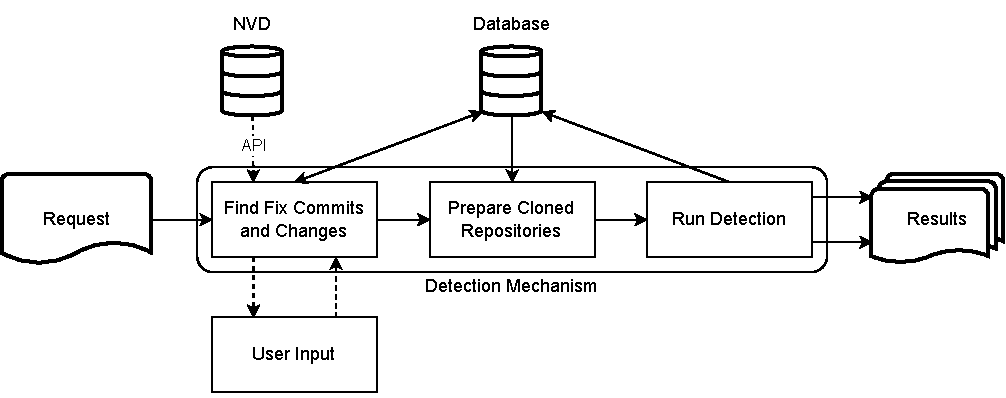
\includegraphics[width=0.95\textwidth]{obrazky-figures/cloneguard_workflow1.drawio.pdf}
    \caption{Basic workflow of the targeted detection scan.}
    \label{cg-workflow1}
  \end{figure}

  \subsection*{Discovery Scan}
  The workflow of the discovery scan is visible in Figure~\ref{cg-workflow2}. It is designed to run in schedules mainly.
  The goal of this mode is to detect new suspicious commits in monitored repositories which might imply
  new vulnerabilities in forked projects.

  On execution, the watched projects are fetched from the database and their repositories are updated to the latest
  version from the remote server using git. The messages of the latest commits are then scanned for the presence
  of any keyword from a~set containing CWE names\footnote{\href{https://cwe.mitre.org/data/definitions/1387.html}{https://cwe.mitre.org/data/definitions/1387.html} -- top 25 most dangerous weaknesses in 2022}.
  Secondly, a~check of affected files by a~commit is performed based on the file extension and path. For example, changes
  in documentation, release notes and tests are filtered out.

  After applying the filters, the resulting list of commits is reported via e-mail notification for each project,
  stored in the database and passed for further evaluation. The goal of the evaluation is to determine
  the complexity of the patch from each commit based on its granularity and spread. The complexity is represented by the number
  of extracted contexts from a~patch. The ones with low complexity
  can be processed automatically, so they are passed to the detection mechanism. In the end, the results
  are stored in the database and are observable in the logs or presented in the web interface.

  \begin{figure}[h]
    \centering
    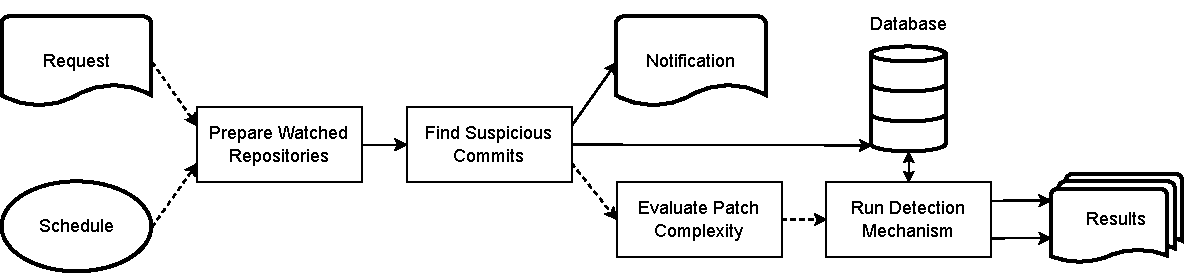
\includegraphics[width=0.95\textwidth]{obrazky-figures/cloneguard_workflow2.drawio.pdf}
    \caption{Workflow of the scheduled vulnerability scan.}
    \label{cg-workflow2}
  \end{figure}

  \section{User Interface}
  \label{design:ui}
  To enhance the user experience and improve overall effectiveness, the tool offers a~graphical interface alongside
  the command line interface. This section will contain a~graphical design of both interfaces, explaining the design choices
  and describing their functionality and use cases. Well designed user interface improves the overall experience with the tool,
  so it is crucial to present the results conveniently.

  \subsection*{Web}
  The graphical user interface (GUI) is accessible via a~web that communicates with the core of the tool
  using an application programming interface (API).
  The web page is organized into three crucial pages. The initial page presents an overview of the current state of the tool.
  Subsequently, a~user can navigate to the second page to initiate and configure the detection process.
  The third page showcases the detection results enabling the user to efficiently analyse and interpret the outcome.
  Additionally, using the tab in the upper right corner user can navigate to the documentation of the API.

  The draft of the page containing an overview of the tool is displayed in Figure~\ref{cg-web-overview}.
  It allows a~user to observe the state of the database, namely registered repositories and stored vulnerability
  records. As was mentioned in the Subsection~\ref{section:targeted-detection}, only registered repositories can be scanned
  by the detection method. Here it is possible to register new repositories to the tool by providing an URL,
  the programming language and the parent of the project in case it was forked from one of the already registered projects. In the second table, the records of previously
  scanned vulnerabilities can be updated to improve the precision and performance of the detection method.
  After updating a~record of the vulnerability it becomes marked as verified. This marking is visible in the last attribute
  of the entity.

  Figure~\ref{cg-web-search} displays the page, where the detection can be started after providing the required
  parameters -- identification of the vulnerability and its source project for the targeted detection.
  The identification of the vulnerability refers to the one stored in the internal database. The parameter \texttt{date}
  is optional. The first step of the detection method is executed using the button \texttt{Search}.
  Accordingly, the results from the search of fix commits are shown below. The list of candidate fix commits is observable
  on the left side of the page. After selecting a~specific commit, the changes from the commit are displayed in the adjacent
  text area. In order to start the clone detection, optionally the patch or code in the middle
  of the page can be edited to contain only code relevant to the fix of the vulnerability. Whether a~patch or code
  segment is required depends on the method which should be used for the detection of clone propagation. In case the search
  is done for a~known and verified vulnerability in the internal database, the stored values are pre-filled in the input
  fields. The button \texttt{Detect} then starts the clone detection.

  \begin{figure}[h]
    \centering
    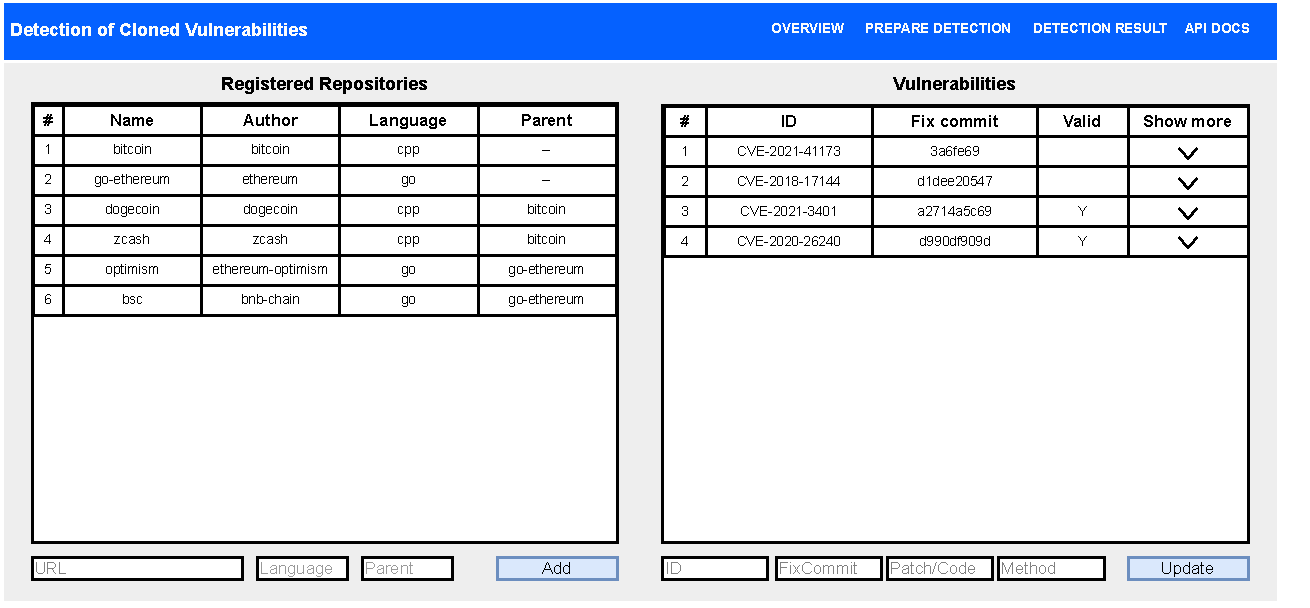
\includegraphics[width=0.95\textwidth]{obrazky-figures/cg_web_overview.drawio.pdf}
    \caption{The design of the page displaying an overview of the state of the tool.}
    \label{cg-web-overview}
  \end{figure}

  \begin{figure}[h]
    \centering
    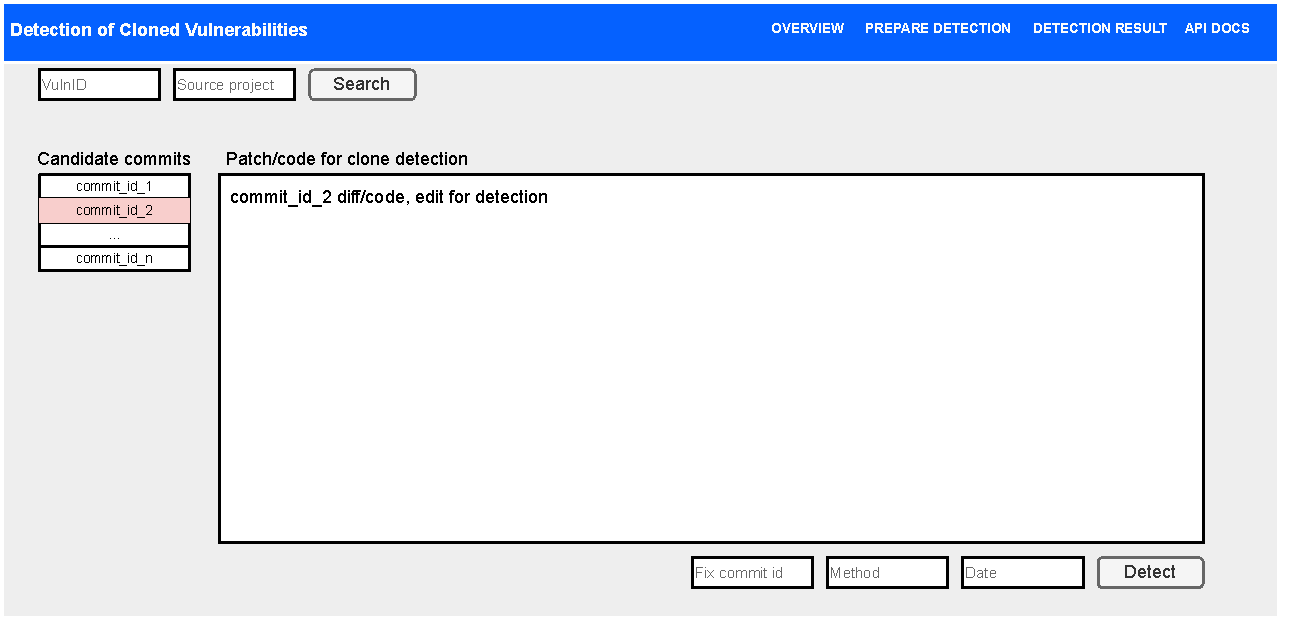
\includegraphics[width=0.95\textwidth]{obrazky-figures/cg_web_search.drawio.pdf}
    \caption{The design of the page where the detection mechanism can be configured and started.}
    \label{cg-web-search}
  \end{figure}

  After the detection is started, the logs and the preliminary results are visible on the last page. The design of this
  page is pictured in Figure~\ref{cg-web-results}. The page is just informative and does not affect the detection.
  The logs contain everything connected to the detection algorithm and the actual results can be hardly visible. To improve the transparency of the results,
   a~list containing a~summary of the detected cloned vulnerabilities is located on the right side. It provides the name of
  the affected project, the confidence of the result and a~reference to the location of the clone in the directory of the project.

  \begin{figure}[h]
    \centering
    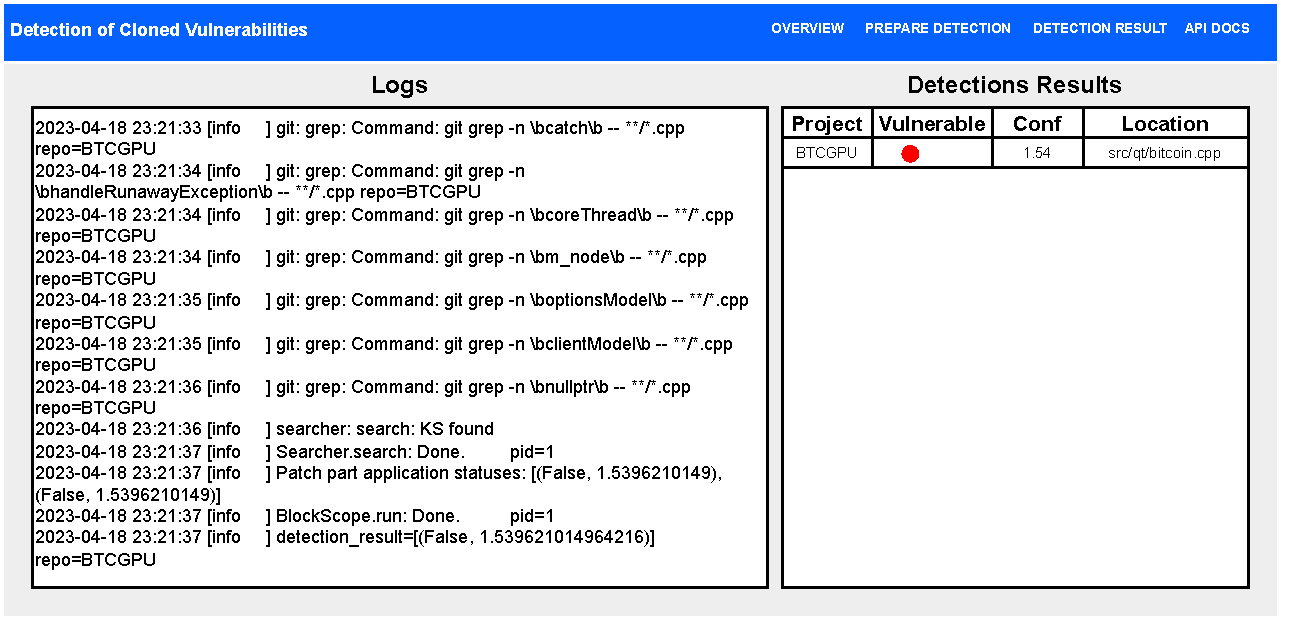
\includegraphics[width=0.95\textwidth]{obrazky-figures/cg_web_results.drawio.pdf}
    \caption{The design of the page displaying the logs and positive detection results.}
    \label{cg-web-results}
  \end{figure} % TODO: location of the candidate

  \subsection*{Command Line Interface}
  The command line interface (CLI) is a~fundamental way to interact with the tool. In comparison to the GUI,
  it offers advantages in terms of speed, customizing and automation. The functionalities allow a~user to:
  \begin{itemize}
    \item register new projects
    \item run the targeted detection
    \item configure schedule of the discovery scan
    \item run a~discovery scan
    \item initialize the schema of the internal database
  \end{itemize}

  In addition to the GUI capabilities, the CLI offers configuration and execution of discovery scan, initialization
  and execution of tests of the detection method. Unlike the GUI, which relies on communication using API, the CLI interacts
  directly with the core of the tool. This dual interface design caters to diverse user preferences, enhancing the overall
  user experience and functionality of the tool.

    % File: src/chapter_5_implementation.tex
% Project: Monitoring and Reporting Tool for Cloned Vulnerabilities across Open-Source Projects
% Author: Matus Remen (xremen01@stud.fit.vutbr.cz)
% Description: Chapter 5 - Implementation

\chapter{Implementation}
\label{chapter:implementation}
  This Chapter outlines the implementation of the tool designed to scan and detect cloned vulnerabilities in open-source projects.
  The tool leverages a~modern technology stack, consisting of Python~3\footnote{\href{https://www.python.org/downloads/}
  {https://www.python.org/downloads/}} for the backend and the API, Redis and PostgreSQL
  for databases and ReactJS for the web interface. Additionally, the entire application is containerized using
  Docker Compose\footnote{\href{https://docs.docker.com/compose/}{https://docs.docker.com/compose/}},
  which offers organized management of multiple services displayed in Figure~\ref{cg-services}.
  By leveraging the mentioned technologies, the tool provides an efficient and user-friendly solution for identifying
  cloned vulnerabilities in open-source software, thus contributing to secure software development practices.

  \begin{figure}[h]
    \centering
    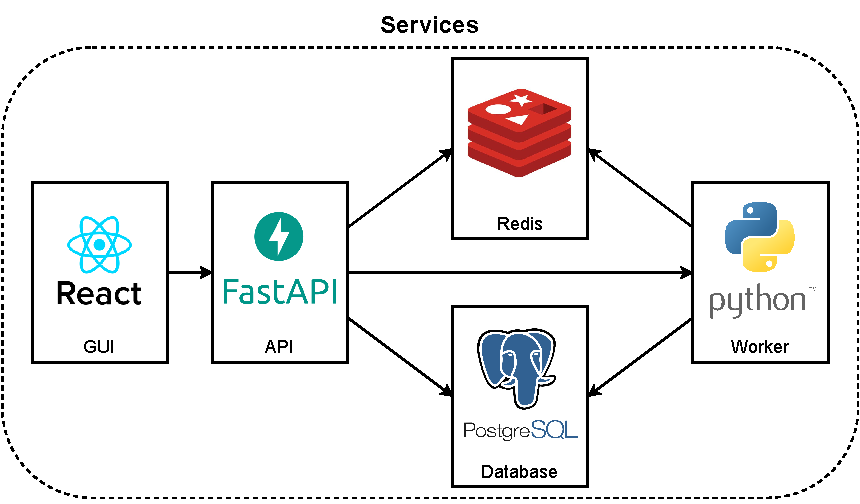
\includegraphics[width=0.7\textwidth]{obrazky-figures/cg_services.drawio.pdf}
    \caption{An overview of the services constructing the tool and their mutual dependencies.}
    \label{cg-services}
  \end{figure}

  For the development of the major part of the tool, Python~3 was chosen, a~versatile and widely used programming language known for its
  readability and ease of use. As the tool uses various technologies, the main benefit of this choice is versatility,
  which assures compatibility between particular parts of the tool and communication with various external APIs.
  In the transition from API to the backend and its detection methods, the choice of Python as the development language
  plays a~significant role in integrating key architectural elements, such as the Redis\footnote{\href{https://redis.io/docs/about/}{https://redis.io/docs/about/}} and
  PostgreSQL\footnote{\href{https://www.postgresql.org}{https://www.postgresql.org}} database. Although, it could suffer
  from execution speed in the case of detection methods in comparison to the programming language C++~\cite{hackrPythonVSCPP}.

  \section{Storage}
  Overall, there are three types of storage used by the tool: the database, the local storage and in-memory storage -- Redis.
  This Section will describe the implementation and usage of each type.

  \subsection*{Database}
  \label{impl:database}
  The internal database is the first type of utilized storage, which is used for storing long-term data, containing
  essential configurations for the tool and results of the detection method. For the implementation of the schema designed
  in Section~\ref{design:database} an open-source object-relational database management system PostgreSQL was selected
  for its great ability to scale. PostgreSQL provides a~docker image, which eases the integration to the tool
  thanks to the usage of containerization via Docker Compose.

  The connection to the database is established using a~Python library \texttt{psycopg2}\footnote{\href{https://www.psycopg.org/docs/}
  {https://www.psycopg.org/docs/}} an efficient, low-level PostgreSQL database adapter performing
  basic database operations. Additionally, an Object Relational Mapper (ORM) library
  \texttt{SQLAlchemy}\footnote{\href{https://www.sqlalchemy.org}{https://www.sqlalchemy.org}}
  is used to simplify access and operations with database objects.
  It provides a~high-level, object-oriented interface that abstracts the underlying database system and allows it to work
  during the development with Python classes instead of raw SQL queries.

  To access the features of the \texttt{SQLAlchemy}, the schema of tables in the database is implemented in Python classes which
  inherit from \texttt{DeclarativeBase} class provided by the library. That defines at once both, the Python object model
  and database metadata that describe tables in the database. According to the designed database schema, the tool implements
  classes \texttt{Bug}, \texttt{Project} and \texttt{Detection} this way.

  To improve readability and developer experience, the tool implements an interface abstracting all operations with the tables
  in the database. The interface is available in a~CRUD module, which implements all used variants of queries to Create, Read,
  Update and Delete records in the database in one place.

  \subsection*{Local Storage}
  \label{impl:local-storage}
  The second type of storage used by the tool is its own local storage on the hosting file system. It is used for storing clones of registered repositories
  and logs from the detection method. During the execution of the detection method, all operations and commands with the analysed
  projects are performed on the clones stored here. By fetching the log files stored here, the API provides data for the page
  displaying detection results in the web interface.

  \subsection*{Redis}
  \label{impl:redis}
  Redis is an open-source, in-memory data structure store used by this tool as a~cache storing a~queue of scheduled
  requests for execution of detection method. As in-memory storage, Redis provides very fast read and write actions,
  and it supports a~wide variety of data structures. Additionally, it is distributed also as a~docker image, which allows
  easy integration of the service using Docker Compose. The connection
  and operations with Redis are assured by a~Python library \texttt{redis}\footnote{\href{https://redis.io/docs/clients/python/}
  {https://redis.io/docs/clients/python/}}.

  To initialize and manage the aforementioned queue in Redis a~Python library \texttt{rq}\footnote{
  \href{https://github.com/rq/rq}{https://github.com/rq/rq}} is used, which stands for Redis Queue. The purpose of this library
  is to schedule jobs for processing in the background and extend the options of the tool in terms of scalability. In the
  implementation of the tool, the jobs are queued by an API and processed by the worker service.

  \section{Detection Mechanism and its Components}
  The detection mechanism is the core component of the tool developed in this project. It is implemented using the programming
  language Python~3 and an object-oriented approach. The mechanism requires on the input an identification of a~bug and the name of the project
  where it was discovered. Accordingly, at the beginning of the workflow, the mechanism finds a~fixing commit of the provided vulnerability,
  parses important details and creates an object representing the bug.

  \begin{figure}[h]
    \centering
    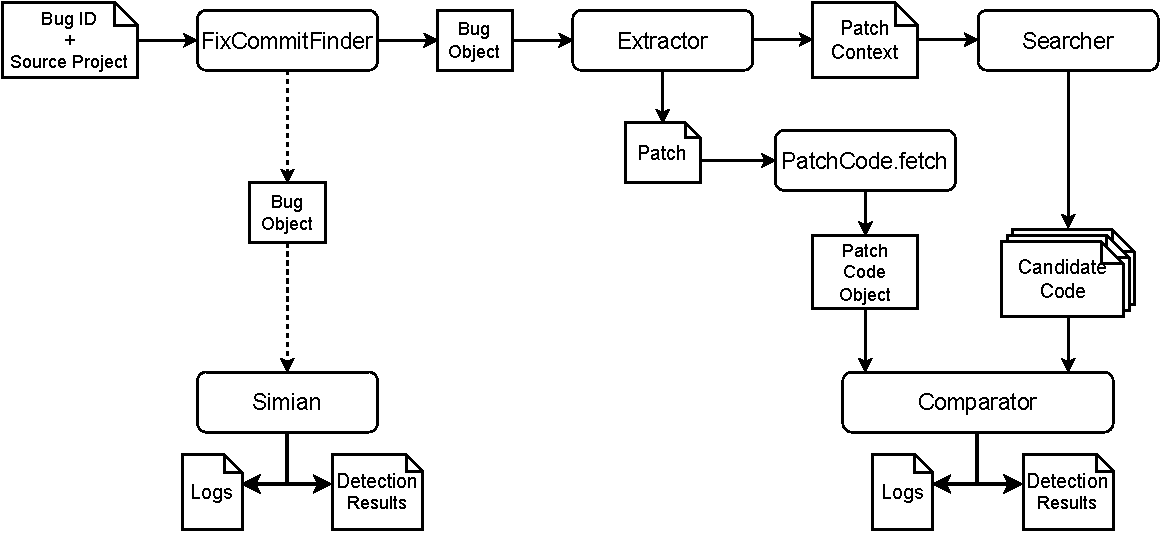
\includegraphics[width=1\textwidth]{obrazky-figures/cg_impl_detection.drawio.pdf}
    \caption{Workflow of the default detection method, with an optional alternative method using tool Simian. Both
             methods process the same Bug Object created after processing the detection request
             specifying the Bug ID and the project where it originated.}
    \label{cg-impl-detection}  % TODO add step with initialization of projects
  \end{figure}

  At this point, the mechanism offers two methods for detecting the propagation of the bug among the forks of the source project.
  The first method utilizes a~tool Simian, which has great performance but is able to detect only clones of the first type.
  The second, default method is inspired by the approach of the tool BlockScope, which is capable of detecting clones of Type~I,
  Type~II and Type~III.

  The complete workflow of the mechanism and its components is displayed in Figure~\ref{cg-impl-detection}. The components
  of the workflow and its implementation will be described in the following subsections.

  \subsection*{Component \texttt{FixCommitFinder}}
  Upon execution of the detection mechanism, the component \texttt{FixCommitFinder} is the first functional part of the workflow.
  It is developed as a~class implementing methods for finding bug-fixing commits for both, the targeted detection
  and discovery scan.

  \begin{figure}[h]
    \centering
    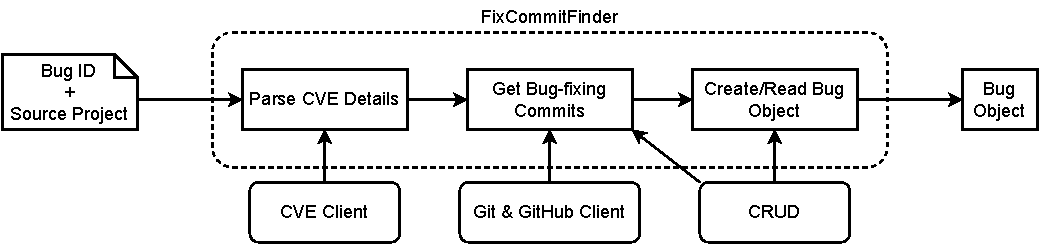
\includegraphics[width=0.9\textwidth]{obrazky-figures/cg_impl_fixcommitfinder.drawio.pdf}
    \caption{Workflow of the component \texttt{FixCommitFinder} in targeted detection. In the case of CVE ID, the component
             parses and uses its details to find bug-fixing commit in the source repository. The fix commits can be supplied
             from the internal database using the CRUD interface.}
    \label{cg-impl-fixcommitfinder}
  \end{figure}

  The process of the component \texttt{FixCommitFinder} in targeted detection is described in Figure~\ref{cg-impl-fixcommitfinder}.
  If the given bug ID is available in the internal database, the final bug object is fetched from there using the CRUD interface
  and returned. Otherwise, if a~CVE is provided, a~class \texttt{CVEClient} is used for parsing its details. The class utilizes a~Python~3 library
  \texttt{requests}\footnote{\href{https://docs.python-requests.org/en/latest/index.html}
  {https://docs.python-requests.org/en/latest/index.html}} for retrieving the data from National Vulnerability Database API using
  HTTP requests. Subsequently, the references to a~fixing commit, pull request or release notes in details about the vulnerability
  are parsed. If the references are not available or recognized, the component additionally extracts keywords from the description
  of the vulnerability using a~library \texttt{nltk}\footnote{\href{https://www.nltk.org}{https://www.nltk.org}}. All extracted details
  are then used for finding the bug-fixing commits using commands of tool \texttt{git}\footnote{\href{https://git-scm.com}
  {https://git-scm.com}} and GitHub API\footnote{\href{https://docs.github.com/en/rest}{https://docs.github.com/en/rest}} available
  in a~class \texttt{Git}. In the end, if the bug ID was not available in the internal database before, the component creates a~new
  object \texttt{Bug}, stores it and returns. A~visualisation of the returned object is available in Figure~\ref{cg-impl-bug-object}.

  \begin{figure}[h]
    \centering
    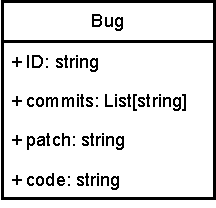
\includegraphics[width=0.25\textwidth]{obrazky-figures/cg_impl_bug_object.drawio.pdf}
    \caption{Overview of the object \texttt{Bug} and its utilized attributes.}
    \label{cg-impl-bug-object}
  \end{figure}

  For the discovery scan, a~different method of the component is used and its workflow is displayed
  in Figure~\ref{cg-impl-fixcommitfinder-scan}. This method requires the on input only the object of the repository
  which will be scanned for new bug-fixing commits for the past couple of days. In the end, this process returns a~list of suspicious
  commits which were detected by a~keywords representing a~software weaknesses or a~patch action in commit messages.

  \begin{figure}[h]
    \centering
    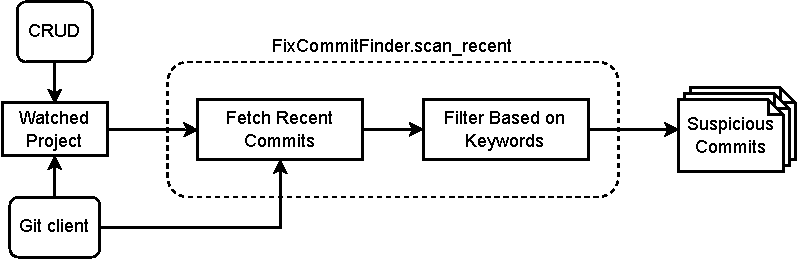
\includegraphics[width=0.9\textwidth]{obrazky-figures/cg_impl_fixcommitfinder_scan.drawio.pdf}
    \caption{Overview of a workflow of the component \texttt{FixCommitFinder} using method for discovery scan.}
    \label{cg-impl-fixcommitfinder-scan}
  \end{figure}

  \subsection*{Component \texttt{BlockScope}}
  The default method of the detection mechanism is based on the approach proposed in the paper about a~tool BlockScope,
  which was described in Section~\ref{section:blockscope}. The implementation of particular components involved in this method
  slightly diverged as it is visible on the right side of Figure~\ref{cg-impl-detection}.

  The component \texttt{Fetcher} from the original design is omitted and its functionality was inherited by the component
  \texttt{Searcher} and a~method of the object \texttt{PatchCode}. It was implemented this way to encapsulate every attribute
  and action related to the patch into one object as during extraction of the patch code is done an additional analysis of structure,
  thus type of the patch is. The component \texttt{Searcher} in this design implements both the context-based search process
  for localization of candidate code in the target repository and extraction of the candidate code.

  Each part of the method produces logs, which can be observed on the web. In the end, if the final result of the detection
  is that the analysed project did not apply the patch, the result is additionally archived in the internal database.

  \subsection*{Component \texttt{Simian}}
  Simian\footnote{\href{https://www.harukizaemon.com/simian}{https://www.harukizaemon.com/simian}} is a~tool for detecting
  code duplicates. It is integrated into the detection mechanism as an alternative method for analysing vulnerable code duplication
  between the source project and its forks. Simian is implemented in the programming language Java, so for its execution was implemented an interface
  as a~separate component, which was named after the tool. The interface also implements a~parser for its output.
  An example output of the tool and parsed information is displayed in Figure~\ref{cg-impl-simian-output}.

  \begin{figure}[h]
    \centering
    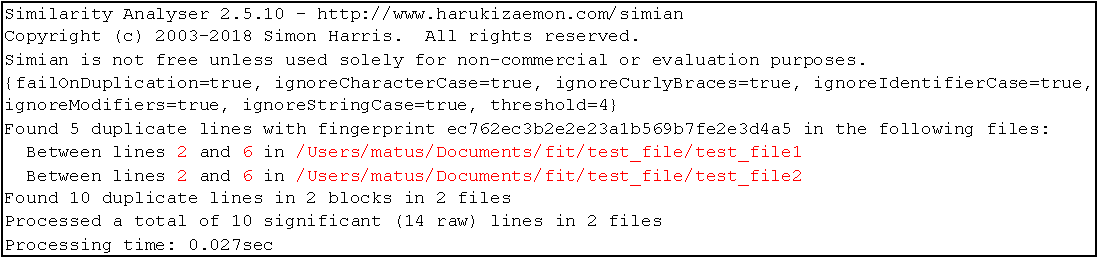
\includegraphics[width=0.9\textwidth]{obrazky-figures/cg_impl_simian_output.drawio.pdf}
    \caption{Output from Simian with highlighted information that is parsed in the detection mechanism.}
    \label{cg-impl-simian-output}
  \end{figure}

  \section{Application Programming Interface}
  The application programming interface (API) is an important part of the tool as it controls communication between the GUI
  and the core of the application. For the implementation of the REST API was chosen Python web framework FastAPI\footnote{
  \href{https://fastapi.tiangolo.com}{https://fastapi.tiangolo.com}}. It achieves great performance, supports
  asynchronous programming and automatically generates API documentation. The implementation of API endpoints
  will be described in the rest of the section.

  \subsection*{API Endpoints}
  \label{impl:api}
  The implemented API contains overall 9 endpoints which deliver messages between the frontend and backend,
  plus one additional which contains the documentation. In the following subsections, each endpoint will be described.
  The documentation of all API endpoints that will be mentioned is accessible
  via the endpoint \texttt{/docs}, in addition to the description, providing also example usage.
  In production, each endpoint has an additional prefix \texttt{/api/v1} which contains a~versioning. It labels
  a~specific version of the software which helps with referencing and tracking changes.

  \subsubsection*{\texttt{GET \ /ping}}
  This endpoint performs a ``health'' check and informs about the status of the API, whether it is running
  and responsive. If there is any issue it is propagated by the HTTP status code representing failure, otherwise the endpoint
  returns the following response: \texttt{\{``pong'':true\}}

  \subsubsection*{\texttt{GET \ /project/fetch\_all}}
  The endpoint \texttt{/project/fetch\_all} is used to fetch all registered projects in the internal database. The possible responses
  when API is running are shown in Table~\ref{tab:project-fetchall}.

  \begin{table}[h]
        \centering
        \begin{tabular}{|c|l|}
          \hline
            HTTP code & Description \\
          \hline
            \texttt{200} & OK -- returns the list of registered projects \\
            \texttt{503} & Resource unavailable error -- DB is not accessible \\
          \hline
        \end{tabular}
        \caption{Overview of responses from API endpoint \texttt{/project/fetch\_all}.}
        \label{tab:project-fetchall}
    \end{table}

  \subsubsection*{\texttt{GET \ /bug/fetch\_all}}
  This endpoint is used to fetch details about all bugs stored in the database, containing their identification,
  fix commit, verification status, patch and code. The responses are listed in Table~\ref{tab:bug-fetchall}.

  \begin{table}[h]
        \centering
        \begin{tabular}{|c|l|}
          \hline
            HTTP code & Description \\
          \hline
            \texttt{200} & OK -- returns list of stored bugs \\
            \texttt{503} & Resource unavailable error -- DB is not accessible \\
          \hline
        \end{tabular}
        \caption{Overview of responses from API endpoint \texttt{/bug/fetch\_all}.}
        \label{tab:bug-fetchall}
    \end{table}

  \subsubsection*{\texttt{POST /project/register}}
  The \texttt{/project/register} endpoint is used to add a~new repository to the database and clone it to the local storage
  of the tool. In order to be able to perform detection in a~repository, firstly it needs to be registered using this endpoint.
  When a~project is successfully registered the API schedules a~task in the Redis Queue~(\ref{impl:redis}) to clone the repository
  in the background process by the service Worker.

  \begin{table}[h]
        \centering
        \begin{tabular}{|c|l|}
          \hline
            Field & Description \\
          \hline
            \texttt{url} & CVS URL to clone the repository from \\
            \texttt{language} & programming language of the project \\
            \texttt{parent} & name of the parent project (optional as it might be the parent) \\
          \hline
        \end{tabular}
        \caption{Overview of request payload fields of API endpoint \texttt{/project/register}.}
        \label{tab:project-register-rq}
    \end{table}

  \begin{table}[h!]
        \centering
        \begin{tabular}{|c|l|}
          \hline
            HTTP code & Description \\
          \hline
            \texttt{201} & Created -- returns details of the registered project \\
            \texttt{422} & Validation error -- some payload fields are missing or invalid \\
            \texttt{503} & Resource unavailable error -- DB is not accessible \\
          \hline
        \end{tabular}
        \caption{Overview of responses from API endpoint \texttt{/project/register}.}
        \label{tab:project-register-rs}
    \end{table}

  The payload of the request always needs to contain fields \texttt{url}, \texttt{language} and \texttt{parent}.
  The description of the request payload fields is available in Table~\ref{tab:project-register-rq} and the responses
  in Table~\ref{tab:project-register-rs}. It is mandatory to specify the cloning
  \texttt{url}\footnote{\href{https://docs.github.com/en/get-started/getting-started-with-git/about-remote-repositories}{https://docs.github.com/en/get-started/getting-started-with-git/about-remote-repositories}}
  in the \texttt{https://} form in order to avoid the need to set up a password-protected SSH key in the worker service, which is needed
  in case of cloning using an SSH URL. During the processing of the request, from the \texttt{url} value is parsed name and owner
  of the project, which are stored in the database using the CRUD interface defined in Section~\ref{impl:database}.

  \subsubsection*{\texttt{POST /bug/update}}
  The endpoint \texttt{/bug/update} is used to specify details about bugs stored in the database, namely the fix
  commits, patch and code attributes. In the case of the detection method using the tool Simian, it is mandatory to specify
  the code to be used for the detection of clones, while the default detection method using the approach of BlockScope
  can extract the patch from the commit automatically. Although to increase the precision of this method, the specifically
  crafted patch can be provided in this way.

  The description of responses and payload fields of this endpoint is described in Table~\ref{tab:bug-update-rs}
  and~\ref{tab:bug-update-rq} respectively. In the payload it is mandatory to specify the field \texttt{id}, \texttt{method}
  and at least one of \texttt{fix\_commit} and \texttt{patch}.

  \begin{table}[h]
        \centering
        \begin{tabular}{|c|l|}
          \hline
            Field & Description \\
          \hline
            \texttt{id} & ID of the bug in the database (e.g. CVE-2021-3401) \\
            \texttt{fix\_commit} & commit hash to be specified as a~bug-fixing commit \\
            \texttt{patch} & base64-encoded patch or code for the specified detection method \\
            \texttt{method} & method specifies whether column \texttt{patch} or \texttt{code} should be updated \\
          \hline
        \end{tabular}
        \caption{Overview of request payload fields of API endpoint \texttt{/bug/update}.}
        \label{tab:bug-update-rq}
    \end{table}

    \begin{table}[h]
        \centering
        \begin{tabular}{|c|l|}
          \hline
            HTTP code & Description \\
          \hline
            \texttt{200} & OK -- returns details of the updated bug \\
            \texttt{404} & Not found error -- the bug with provided ID was not found in the DB \\
            \texttt{422} & Validation error -- some payload fields are missing or invalid \\
            \texttt{503} & Resource unavailable error -- DB is not accessible \\
          \hline
        \end{tabular}
        \caption{Overview of responses from API endpoint \texttt{/bug/update}.}
        \label{tab:bug-update-rs}
    \end{table}

  \subsubsection*{\texttt{POST /detection/search}}
  This endpoint performs a~search of bug-fixing commit candidates of the requested vulnerability in the provided source repository
  where it originated. If the bug is stored in the internal database, the details about it are provided from there.
  Additionally, if the bug has specified a~patch, it is also provided in the response. The description of the payload fields
  are shown in Table~\ref{tab:detection-search-rq} and responses in Table~\ref{tab:detection-search-rs}.

  \begin{table}[h]
        \centering
        \begin{tabular}{|c|l|}
          \hline
            Field & Description \\
          \hline
            \texttt{bug\_id} & ID of the bug in the database (e.g. CVE-2021-3401) \\
            \texttt{project\_name} & project where the bug was discovered \\
          \hline
        \end{tabular}
        \caption{Overview of request payload fields of API endpoint \texttt{/detection/search}.}
        \label{tab:detection-search-rq}
    \end{table}

    \begin{table}[h!]
        \centering
        \begin{tabular}{|c|l|}
          \hline
            HTTP code & Description \\
          \hline
            \texttt{200} & OK -- returns list of candidate commits and patch if available \\
            \texttt{422} & Validation error -- some payload fields are missing or invalid \\
            \texttt{500} & Internal server error -- failed repository initialization or search \\
            \texttt{503} & Resource unavailable error -- DB is not accessible \\
          \hline
        \end{tabular}
        \caption{Overview of responses from API endpoint \texttt{/detection/search}.}
        \label{tab:detection-search-rs}
    \end{table}

  \subsubsection*{\texttt{POST /detection/show\_commit}}
  The purpose of this endpoint is to provide the content of the given commit hash (SHA-1) in the specified project.
  That is useful mainly when multiple candidate commits were found for a~vulnerability, so the user can
  display the content of each candidate and so help with specifying the correct one, which should be further analysed.
  The request payload and the responses from this endpoint are shown in tables~\ref{tab:detection-show-rq} and~\ref{tab:detection-show-rs}
  respectively.

  \begin{table}[h]
        \centering
        \begin{tabular}{|c|l|}
          \hline
            Field & Description \\
          \hline
            \texttt{project\_name} & project where the commit should be searched \\
            \texttt{commit} & commit hash to search \\
          \hline
        \end{tabular}
        \caption{Overview of request payload fields of API endpoint \texttt{/detection/show\_commit}.}
        \label{tab:detection-show-rq}
    \end{table}

    \begin{table}[h]
        \centering
        \begin{tabular}{|c|l|}
          \hline
            HTTP code & Description \\
          \hline
            \texttt{200} & OK -- returns the content of the given commit \\
            \texttt{404} & Not found error -- the commit was not found in the given repository \\
            \texttt{422} & Validation error -- payload field missing or the project is not registered \\
            \texttt{500} & Internal server error -- project initialization or search of commit failed \\
            \texttt{503} & Resource unavailable error -- DB is not accessible \\
          \hline
        \end{tabular}
        \caption{Overview of responses from API endpoint \texttt{/detection/show\_commit}.}
        \label{tab:detection-show-rs}
    \end{table}

  \subsubsection*{\texttt{POST /detection/execute}}
  The endpoint \texttt{/detection/execute} schedules a~detection method execution task to the Redis Queue~(\ref{impl:redis}),
  which is processed in a~background process by the service Worker. Before the detection method is started, the run-time
  logs are forwarded to a~log file located in the local storage~(\ref{impl:local-storage}) of the tool.

  Table~\ref{tab:detection-execute-rq} contains description of the required payload fields and Table~\ref{tab:detection-execute-rs}
  shows responses returned by this endpoint. In the case of the detection method based on BlockScope, one of the fields
  \texttt{commit} and \texttt{patch} needs to be specified, while in the case of the detection method using an integrated tool Simian
  strictly requires the code chunk to be detected. The field \texttt{patch} is used for transferring both the patch for BlockScope
  and the code chunk for Simian.

  \begin{table}[h]
        \centering
        \begin{tabular}{|c|l|}
          \hline
            Field & Description \\
          \hline
            \texttt{bug\_id} & investigated bug ID \\
            \texttt{project\_name} & parent project of analysed cloned repositories \\
            \texttt{commit} & bug fixing commit \\
            \texttt{patch} & base64-encoded patch or code to be detected \\
            \texttt{method} & detection method to be used \\
            \texttt{date} & version of the project from the date which should be considered \\
          \hline
        \end{tabular}
        \caption{Overview of request payload fields of API endpoint \texttt{/detection/execute}.}
        \label{tab:detection-execute-rq}
    \end{table}

    \begin{table}[h!]
        \centering
        \begin{tabular}{|c|l|}
          \hline
            HTTP code & Description \\
          \hline
            \texttt{201} & Created -- task successfully scheduled \\
            \texttt{422} & Validation error -- payload field missing \\
            \texttt{503} & Resource unavailable error -- Redis not available \\
          \hline
        \end{tabular}
        \caption{Overview of responses from API endpoint \texttt{/detection/execute}.}
        \label{tab:detection-execute-rs}
    \end{table}

  \subsubsection*{\texttt{GET \ /detection/status}}
  This endpoint fetches the latest log file from the local storage~(\ref{impl:local-storage}) and provides its content.
  Additionally, the specific detection results are parsed from the logs using regular expressions from Python built-in
  library \texttt{re}\footnote{\href{https://docs.python.org/3/library/re.html}{https://docs.python.org/3/library/re.html}}.
  a~description of possible responses from the endpoint is available in Table~\ref{tab:detection-status-rs}.

  \begin{table}[h]
        \centering
        \begin{tabular}{|c|l|}
          \hline
            HTTP code & Description \\
          \hline
            \texttt{200} & OK -- returns log and parsed detection results \\
            \texttt{500} & Internal server error -- log parsing failed \\
            \texttt{503} & Resource unavailable error -- log file not available \\
          \hline
        \end{tabular}
        \caption{Overview of responses from API endpoint \texttt{/detection/status}.}
        \label{tab:detection-status-rs}
    \end{table}

  \section{User Interfaces}
  This Section provides an implementation overview of available user interfaces, designed in the previous Chapter~\ref{design:ui}.
  The tool provides in total two user interfaces -- web and command line interface. In sections about each, the used technologies,
  libraries and a preview of the results will be mentioned and displayed.

  \subsection*{Web}
  The web is the first available user interface implemented to simplify the usage of the tool in an intuitive manner. For implementation
  was chosen React\footnote{\href{https://react.dev}{https://react.dev}}, an open-source JavaScript library for building user
  interfaces from individual pieces called components. React is free to use and has available a large number of open-source
  libraries which provide pre-built components. For building the web interface was used the React component library
  \texttt{MaterialUI}\footnote{\href{https://mui.com/material-ui/getting-started/overview/}
  {https://mui.com/material-ui/getting-started/overview/}}, which accelerated and simplified the development.

  The preview of the page which displays tables with lists of registered projects and stored bugs in the internal database is available
  in Figure~\ref{cg-impl-overview}. Upon loading, the page requests the lists of projects and bugs from the API
  endpoints \texttt{/project/fetch\_all} and \texttt{/bug/fetch\_all}. In the meantime, the page is rendered and once the API
  provides the requested data it is filled in the tables. To register a~new project the form under the table \texttt{Projects}
  is used and upon submitting, the inputs are processed by the API endpoint \texttt{/project/register}. Likewise, the bugs
  can be updated utilizing the API endpoint \texttt{/bug/update}.

  The second page prepares and executes the detection methods. The preview is available in Figure~\ref{cg-impl-search}.
  Providing the ID of vulnerability and source project name, clicking on the button \texttt{Search}, the web utilizes
  the API endpoint \texttt{/detection/search} to retrieve the list of candidate bug-fixing commits and the patch of the bug,
  if it is available in the internal database. Otherwise, the backend tries to parse it from the details of the given vulnerability.
  In case the list of candidate commits contains multiple results, their contents can be displayed by selecting the desired
  commit. Accordingly, the content of the commit is retrieved from API endpoint \texttt{/detection/show\_commit} and displayed
  in the text area in the middle of the page, which can be manually edited to contain only relevant changes. The fix commit
  in the input field at the bottom of the page is automatically filed according to the selection in the list of candidate commits
  but can be also manually edited. Optionally, the method and date of the repository inputs can be specified before executing
  the detection method. Upon submitting the form using the button \texttt{Detect}, the API endpoint \texttt{/detection/execute}
  is utilized to schedule the targeted detection task and the user is automatically navigated to the page displaying the detection
  log and results.

  \begin{figure}[h]
    \centering
    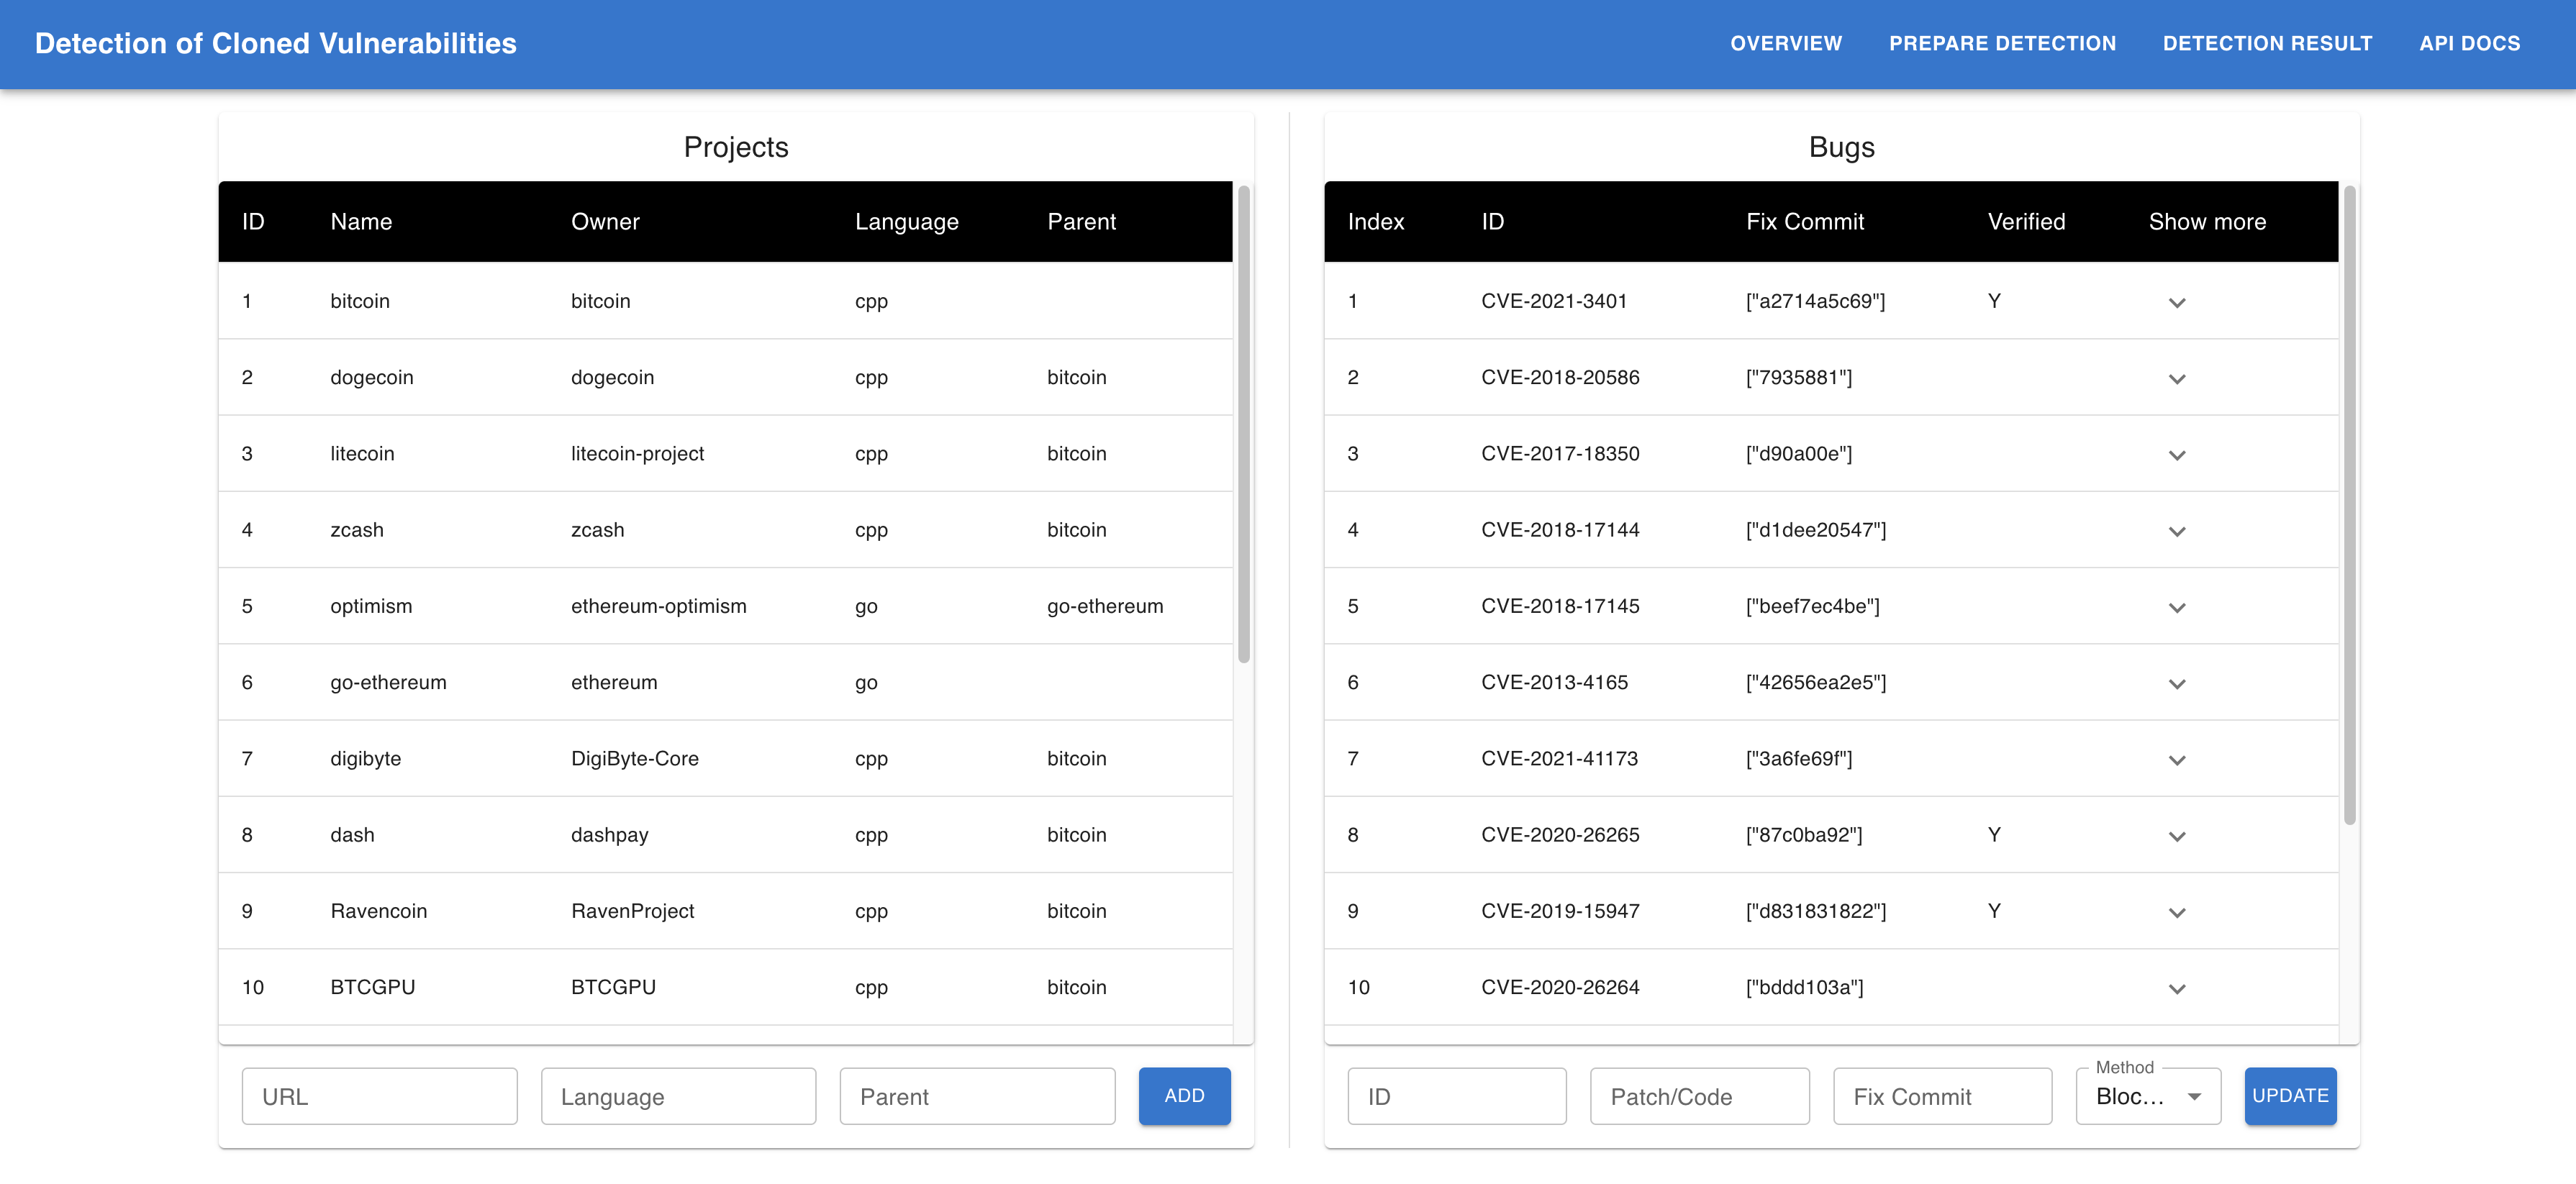
\includegraphics[width=1\textwidth]{obrazky-figures/cg_web_overview.png}
    \caption{Implemented overview web page.}
    \label{cg-impl-overview}
  \end{figure}

  \begin{figure}[h]
    \centering
    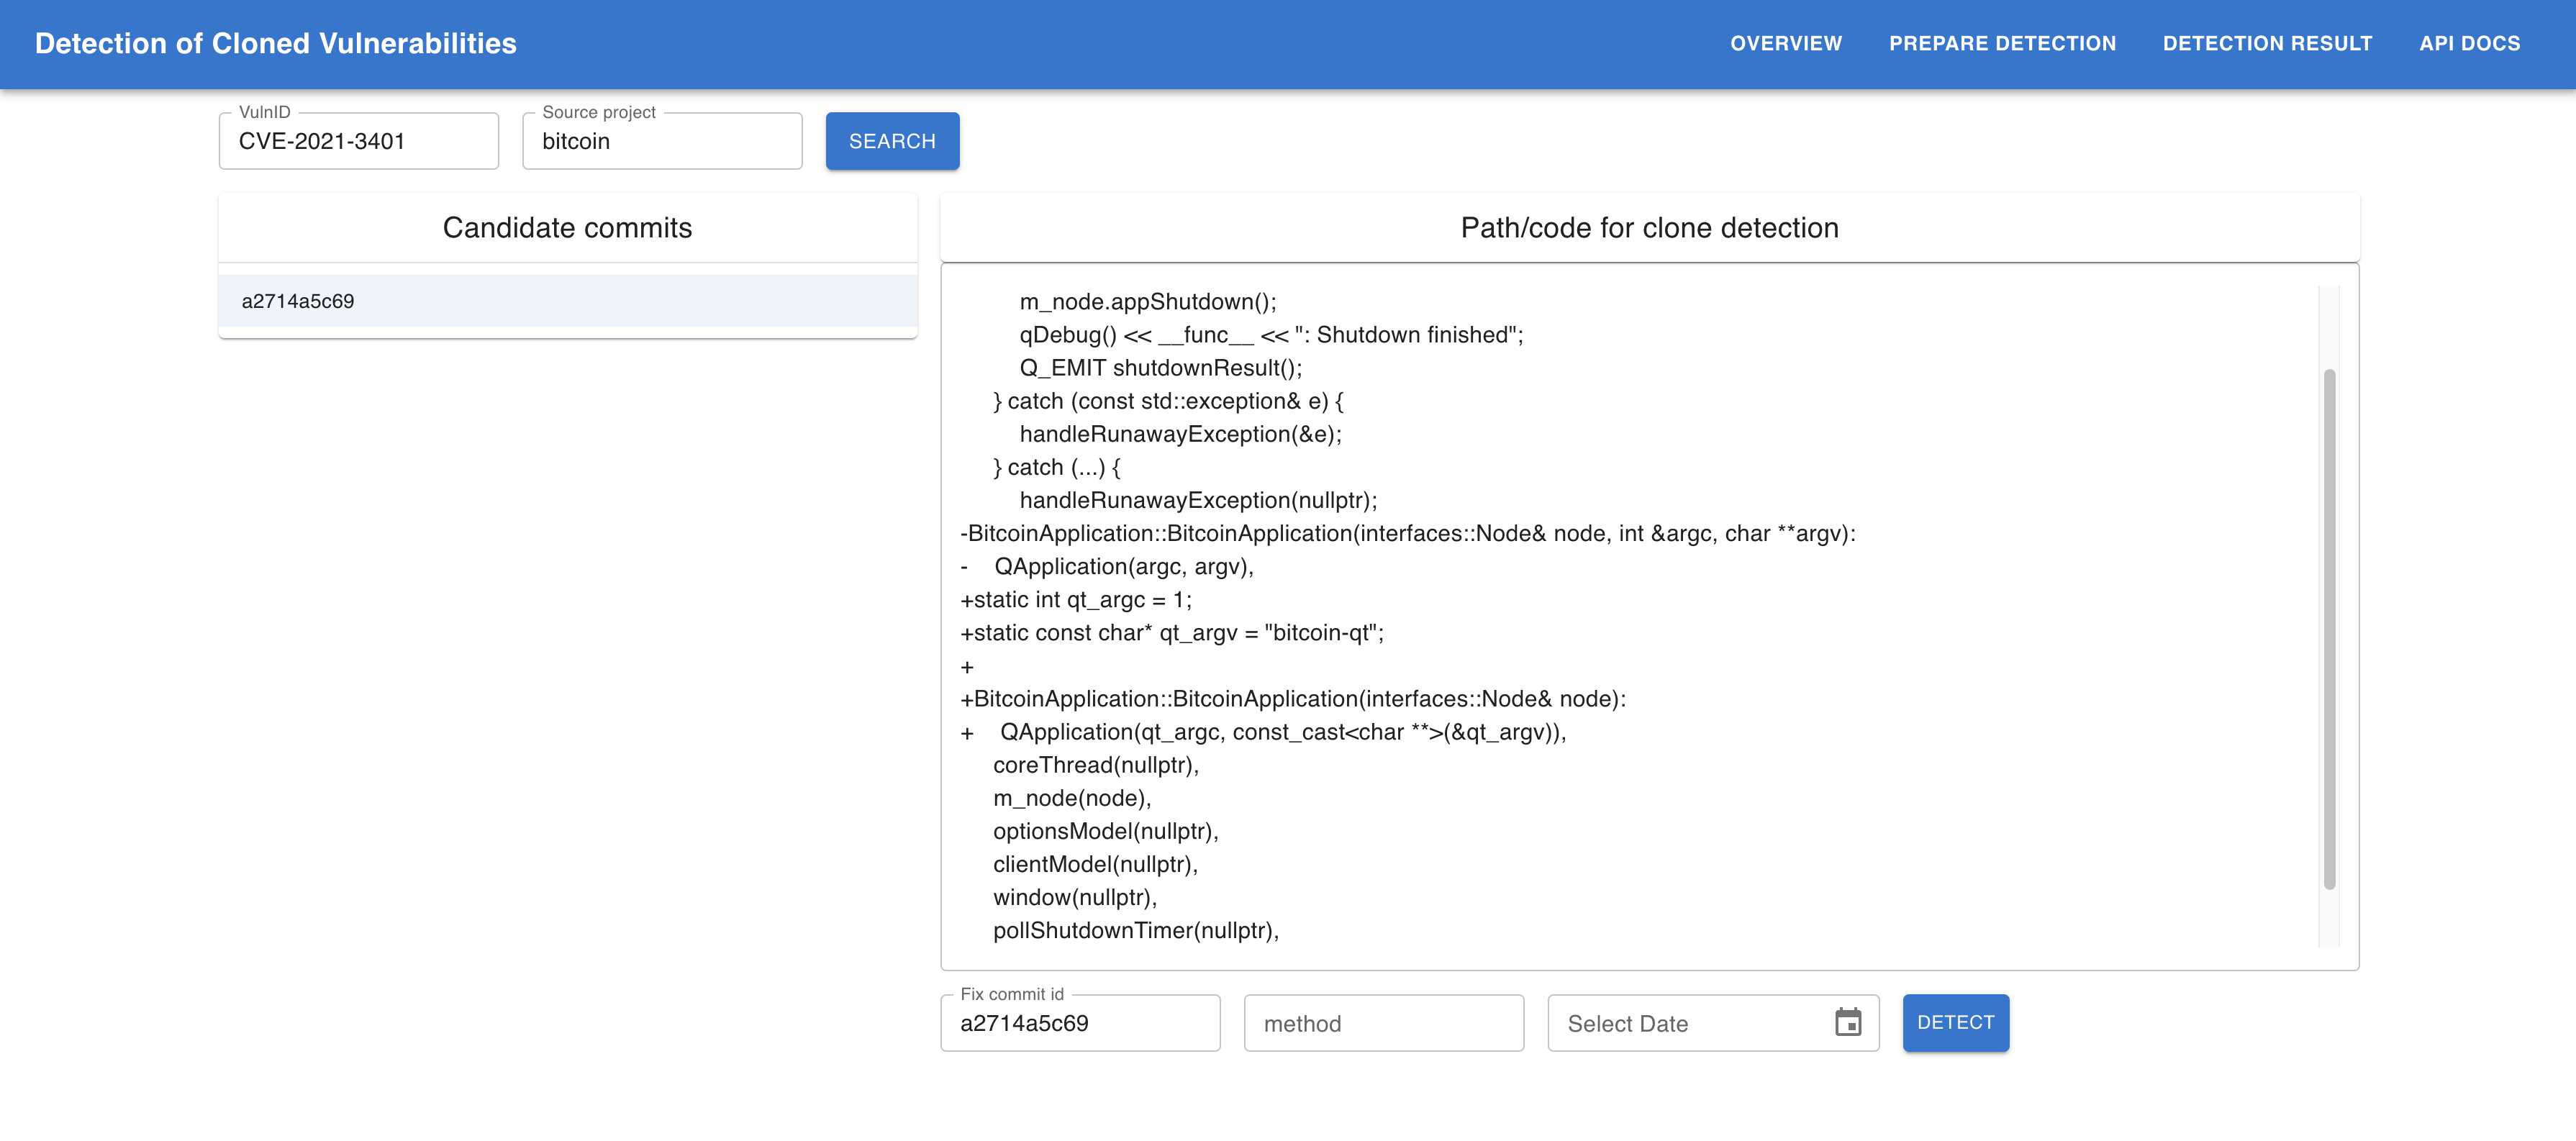
\includegraphics[width=1\textwidth]{obrazky-figures/cg_web_search.png}
    \caption{Implemented prepare detection web page.}
    \label{cg-impl-search}
  \end{figure}

  The preview of the third page is observable in Figure~\ref{cg-impl-results}. The page displays log and parsed results
  from detection method run-time. To fetch required data the web uses the API endpoint \texttt{/detection/results}. The purpose of this page is informational and does not affect the method.

  \begin{figure}[h]
    \centering
    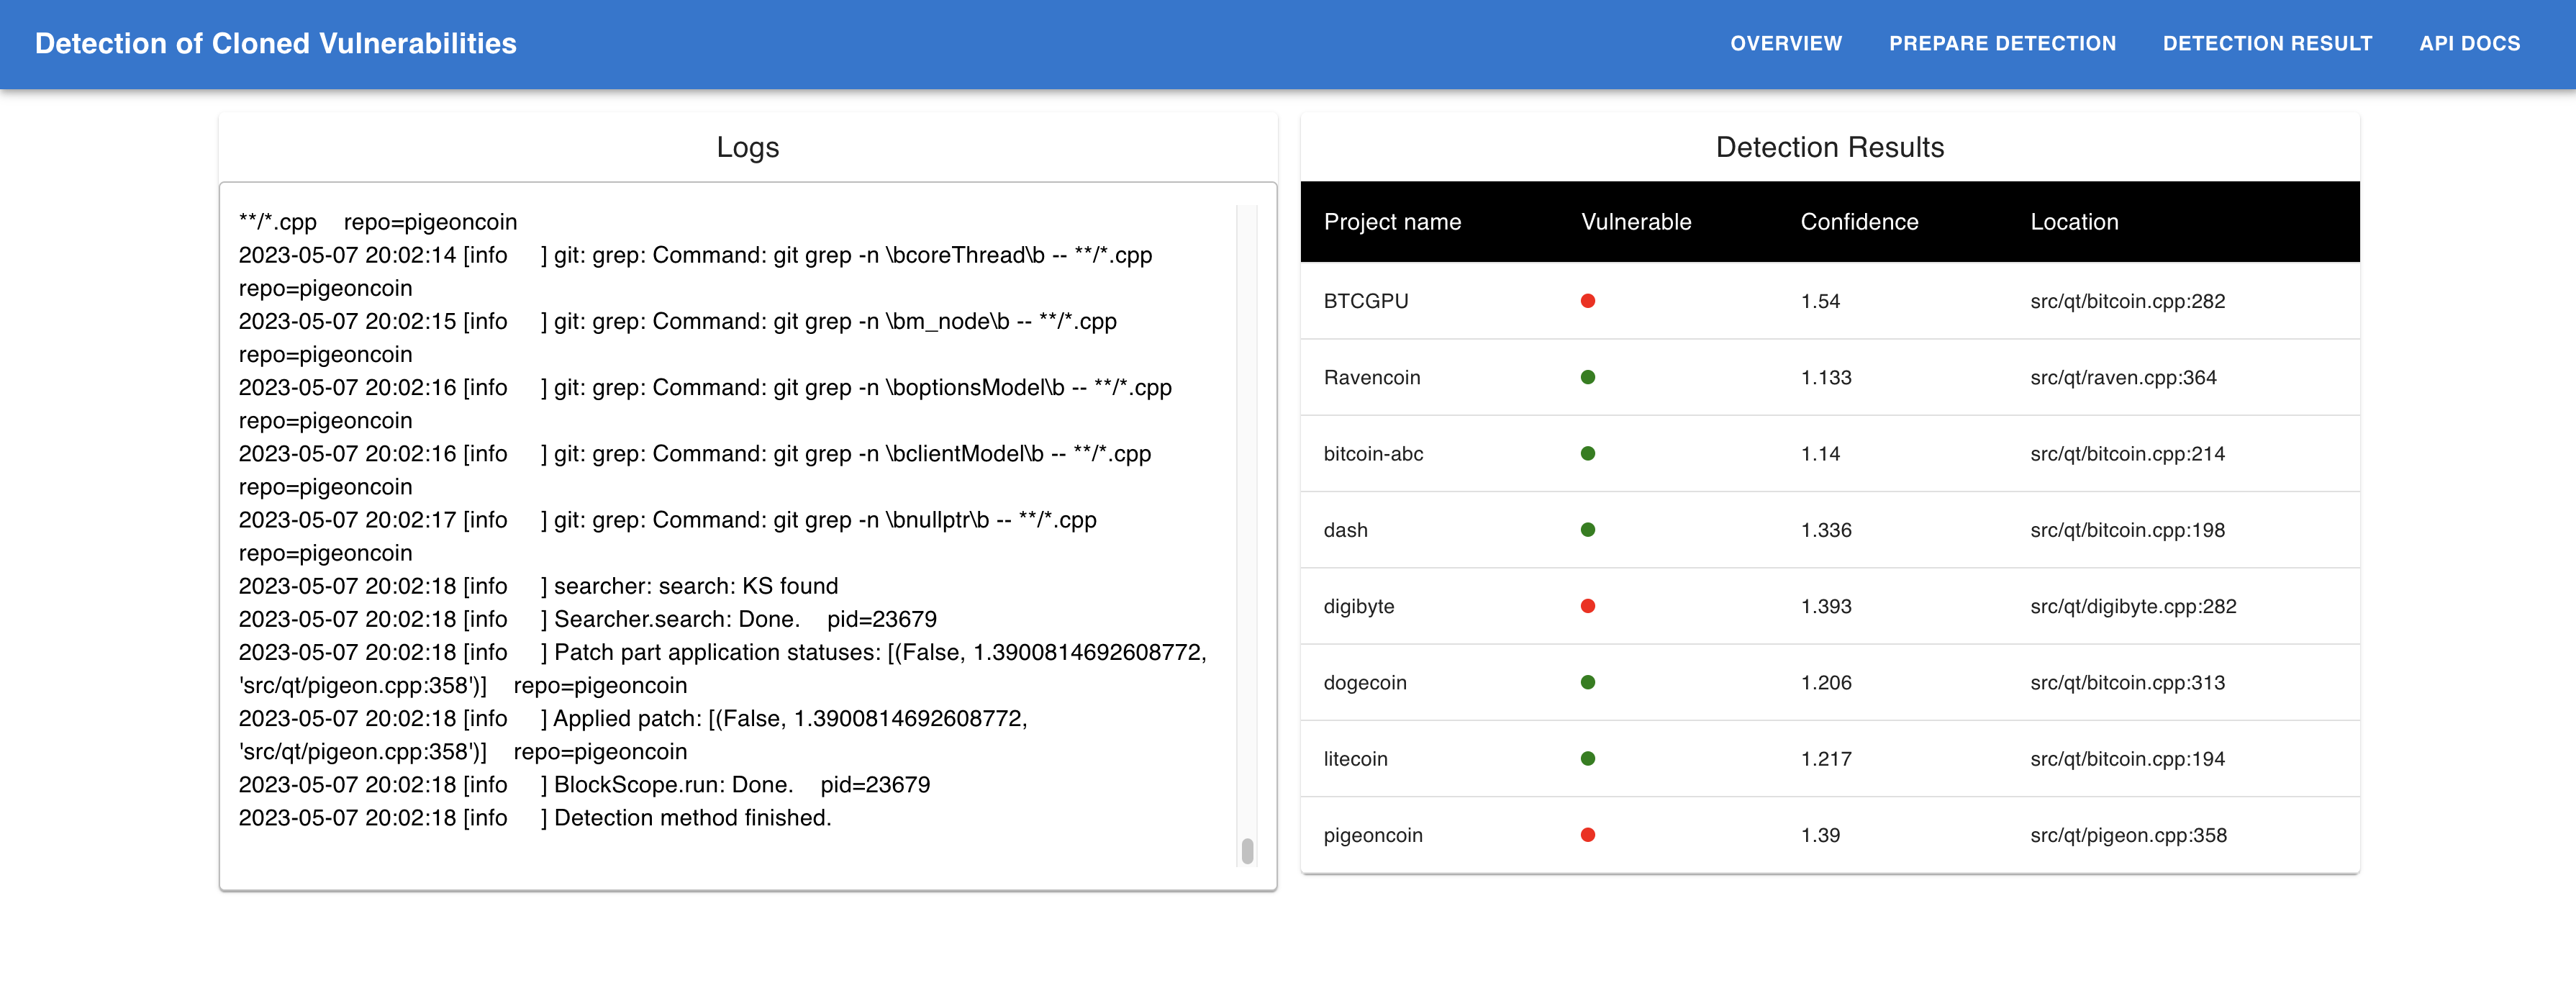
\includegraphics[width=1\textwidth]{obrazky-figures/cg_web_results.png}
    \caption{Implemented web page displaying detection logs and results of CVE-2021-3401.}
    \label{cg-impl-results}
  \end{figure}

  \subsection*{Command Line Interface}
  Additionally to the web, the tool provides also a command line interface (CLI), which benefits in terms of efficiency
  and lesser load on a~machine as it depends only on the database and Redis. Although, the output is not as clear as in the web interface
  and requires an experience with the command prompt.

  For implementation of the CLI a~Python library \texttt{click}\footnote{\href{https://click.palletsprojects.com/en/8.1.x/}
  {https://click.palletsprojects.com/en/8.1.x/}} was used. Its syntax reminds of the FastAPI as the commands and their arguments
  are defined using decorators. The decorators take care of parsing arguments, which makes the code shorter and more clear
  in comparison to other libraries, for example, Python built-in library \texttt{argparse}\footnote{\href{
  https://docs.python.org/3/library/argparse.html}{https://docs.python.org/3/library/argparse.html}}.

  The CLI implements the following commands, which are expecting the same values of arguments as in API:
  \begin{itemize}
      \item register and clone a~new project\\
      \texttt{\$ cli register <URL> <language> [\texttt{-}\texttt{-}parent <project>]}
      \item run targeted detection\\
      \texttt{\$ cli run <bug\_id> <project> <method> [\texttt{-}\texttt{-}date <date>]}
      \item run discovery scan with the option to set a~schedule for scans\\
      \texttt{\$ cli scan [schedule]}
      \item initialize the schema of the database \\
      \texttt{\$ cli db-init}
  \end{itemize}

    % File: src/chapter_6_experimentation.tex
% Project: Monitoring and Reporting Tool for Cloned Vulnerabilities across Open-Source Projects
% Author: Matus Remen (xremen01@stud.fit.vutbr.cz)
% Description: Chapter 6 - Experimentation

\newcommand{\stimes}{\ensuremath{\times}}

\chapter{Experimentation}
\label{chapter:experimentation}
This chapter presents and evaluates the capabilities of the implemented tool. The first section describes the preparation steps,
including system configuration and data set. Then the results produced by the implemented tool are presented in the following
section. Finally, the last section summarizes the results, discusses shortcomings and provides suggestions for possible
improvements and next development.

\section{Preparation}
Initially, the open-source projects \emph{Bitcoin} and \emph{Go-Ethereum} were selected for experiments because of their
popularity, according to the list of cryptocurrencies from the website \emph{CoinGecko}\footnote{\href{https://www.coingecko.com}
{https://www.coingecko.com}}.
The projects were then registered in the internal database as parent projects and their repositories were cloned to the local
storage. From the previously mentioned list of cryptocurrencies and based on prior research, projects which adopted source
code from either \emph{Bitcoin} or \emph{Go-Ethereum} repositories were identified. Accordingly, the identified projects were
registered in the internal database as their forks and cloned to the local storage.

The data set used for experimentation consists of vulnerabilities with assigned CVE identifiers, discovered in the selected parent
projects \emph{Bitcon} and \emph{Go-Ethereum}. The vulnerabilities were selected based on the availability of information about
them, mainly references to patches in order to work with verified data. Accordingly, the web interface was used to create
entities of the bugs in the internal database and attempt to find bug-fixing candidate commits using the functionality of the
component \texttt{FixCommitFinder}. The found candidate commits were then manually validated and the bug-fixing code changes were
extracted, in order to use in the detection method only changes that address patch of the vulnerability. The extracted code
changes were then used to update the corresponding attributes of the bug entity in the internal database, in order to allow
this step to be omitted in the subsequent repeated executions of the detection.

The docker environment was configured to use 4~CPU cores to take advantage of implemented multiprocessing features which
improve the speed of the algorithm and 8~GB of memory for the experimentation. For particular evaluations, the web interface
was used to execute both detection methods for each vulnerability from the prepared data set. Consequently, the detection
results were noted and manually verified in the corresponding code bases in order to evaluate the precision of the implemented
detection methods. Manual verification is needed because the results might contain false detections.

\section{Results}
This section presents the detection results for the prepared list of vulnerabilities. Selected vulnerabilities are closely
analysed to address the capabilities and shortcomings of particular implemented detection methods, while the others provide
only numbers of positive/negative results for the calculation of the success rate.
The detailed results are compared to the expected outcome of the tool and are presented in tables, where a check mark (\checkmark)
represents detected patch, a cross (\stimes) represents that patch was not applied but the vulnerable code detected and an empty
cell means that the clone was not found and vulnerability was not propagated. The results, which do not correspond to reality
(false positives/negatives) are marked by the red color of the cell. The tables display results from the main detection method,
which is based on the approach of BlockScope.

\subsection*{Bitcoin-based vulnerabilities}
A~vulnerability with identifier CVE-2021-3401\footnote{\href{https://nvd.nist.gov/vuln/detail/CVE-2021-3401}
{https://nvd.nist.gov/vuln/detail/CVE-2021-3401}} was selected for the first experiment, as it is the latest published
vulnerability according to the list\footnote{\href{https://en.bitcoin.it/wiki/Common_Vulnerabilities_and_Exposures}
{https://en.bitcoin.it/wiki/Common\_Vulnerabilities\_and\_Exposures}} of weaknesses in \emph{Bitcoin}. The vulnerability was discovered
in the project \emph{Bitcoin} and might allow an attacker to execute arbitrary code upon passing a~malicious argument
to the \texttt{bitcoin-qt} program. This was caused by misuse of built-in arguments of GUI framework Qt\footnote{\href{
https://www.qt.io}{https://www.qt.io}}.

% BTC sv, zen - clones of zcash
\begin{table}[h]
  \centering
  \begin{tabular}{|l|c|c|c|}
    \hline
    CVE-2021-3401 & \multicolumn{3}{|c|}{Patch application status over date} \\
    \hline
    \multicolumn{1}{|c|}{Project} & 21/02/04\ & 22/05/06\ & 23/05/03 \\
    \hline
    bitcoin-abc & \checkmark & \checkmark & \checkmark \\  % T III & T III & T III
    \hline
    bitcoin-sv & & & \\
    \hline
    BTCGPU & \stimes & \stimes & \stimes \\  % T I & T I & T I
    \hline
    dash & \stimes & \checkmark & \checkmark \\  % T I & T II & T II
    \hline
    dogecoin & \stimes & \checkmark & \checkmark \\  % T III & T II & T II
    \hline
    litecoin & \checkmark & \checkmark & \checkmark \\  % T I & T II & T II
    \hline
    pigeoncoin & \stimes & \stimes & \stimes \\  % T III & T III & T III
    \hline
    Ravencoin & \stimes & \stimes & \checkmark \\  % T III & T III & T II
    \hline
    qtum & \checkmark & \checkmark & \cellcolor{red!25} \\  % T I & T I & T II
    \hline
    zcash & & & \\
    \hline
    zen & & & \\
    \hline
  \end{tabular}
  \caption{Detection results for CVE-2021-3401 over various versions of the analysed projects.}
  \label{tab:results-cve-3401}
\end{table}

The results in Table~\ref{tab:results-cve-3401} show that the vulnerability was propagated to some clones of the project Bitcoin.
It contains patch application status for three different states of the projects according to the timeline of each project.
The first, the 4th of February 2021 refers to the date of CVE publishing, and the following display patching progress over time
with the last date, the 3rd of May 2023, referring to the date of this experiment. The results contain the detection of the first
three types of clones -- Type~I, Type~II and Type~III.

Projects \emph{bitcoin-abc}, \emph{dogecoin}, \emph{pigeoncoin} and \emph{Ravencoin} contained clones of Type~III. Clones of
Type~II were found in projects \emph{dash}, \emph{dogecoin} and \emph{Ravencoin} after applying patch and the rest were Type~I
clones. Projects \emph{bitcoin-sv}, \emph{zcash} and \emph{zen} did not adopt the vulnerable code. Although, there was one
miss in case of the project \emph{qtum} in the most recent version, where the upper candidate context was missing, thus the
candidate code was not identified, even when the lower context would be found.

The tool Simian was able to detect vulnerability only in the project \emph{BTCGPU} containing Type~I clone, when run with code
fragment containing the vulnerable version of the code on version from 3rd of May 2023. With version from 4th of February 2021
it was additionally able to detect the vulnerability only in project \emph{dash}, still missing the other three affected projects.

% 23/05/03
% valid - BTCgold - T I
% valid - doge, dash, litecoin, raven-qt - T II
% valid - pigeon, BTCabc,  - T III missing params, reordered params
% invalid - qtum - upper ctx diverged, patch applied T II - qtum-qt
% 23/05/03 BTCsv, zcash, zen -- no Qt at all
% Simian - detected only BTCGPU
% Simian - no support for Go

% 22/05/06
% valid BTCabc, BTCgold, doge, dash, litecoin, pigeon, qtum
% valid Raven - T II
% SIMIAN detected only BTCGPU

% 21/02/04
% digi T II valid - not applied

\begin{table}[h]
  \centering
  \begin{tabular}{|l|c|c|c|}
    \hline
    CVE-2018-17144 & \multicolumn{3}{|c|}{Patch application status over date} \\
    \hline
    \multicolumn{1}{|c|}{Project} & 18/09/14 & 18/09/19 & 23/05/03 \\
    \hline
    bitcoin-abc & & &  \\  % no clone
    \hline
    bitcoin-sv & & & \\  % no clone
    \hline
    BTCGPU & \stimes & \checkmark & \checkmark \\  % T I & & T I
    \hline
    dash & \cellcolor{red!25} &  & \checkmark \\  % T I & T III/IV? & T III fixed?
    \hline
    dogecoin & \stimes & \checkmark & \checkmark \\  % T I & & T I & T I
    %\hline
    %digibyte & \stimes & \stimes & \checkmark \\  % T I
    \hline
    litecoin & \stimes & \checkmark &  \\  % T I & T I
    \hline
    pigeoncoin & \cellcolor{red!25} & \cellcolor{red!25} & \cellcolor{red!25}\stimes \\  % T I
    \hline
    Ravencoin & \stimes & \checkmark &  \\  % T III & T III &
    \hline
    qtum & \cellcolor{red!25} & \checkmark & \\  % T I & T I
    \hline
    zcash & \cellcolor{red!25} & & \\  % T III
    \hline
    zen & \cellcolor{red!25} & & \\  % T III
    \hline
  \end{tabular}
  \caption{Detection results for CVE-2018-17144 over various versions of the analysed projects.}
  \label{tab:results-cve-17144}
\end{table}

An \emph{Inflation bug} was chosen for the second detailed experiment. The bug was discovered alongside Denial-of-Service weakness
in \emph{Bitcoin} and was described in Section~\ref{sec:example-cloned-vuln}. The vulnerability was assigned the identifier
CVE-2018-17144\footnote{\href{https://nvd.nist.gov/vuln/detail/CVE-2018-17144}{https://nvd.nist.gov/vuln/detail/CVE-2018-17144}}.
The experiments were done with various versions of the projects and the most interesting are contained
in Table~\ref{tab:results-cve-17144}. The dates in the table refer to the date before publication of the CVE record, the date
of publication and the date of experimentation.

The results of the tool on this vulnerability are worse in comparison to the previous vulnerability. The reason is that the projects where
the clone was not detected used a version where the context of the vulnerable code contained too many adjustments (\texttt{d1dee20547}) despite the affected code being present. Simian detected additionally
the flaw in projects \emph{dash} and \emph{pigeoncoin}, although missed \emph{Ravencoin} which contained a clone of Type~III
on the 14th of September 2018. On the other side, projects \emph{bitcoin-abc} and \emph{bitcoin-sv} did not clone the affected
code.

To the 3rd of May 2023, most of the repositories already patched the vulnerability using different solutions, thus syntactical
clones were mostly not found, which makes the original patch outdated. Additionally, the original patch contained a~change only on
a single line of code\footnote{\href{https://github.com/bitcoin/bitcoin/pull/14249/commits/d1dee20547}
{https://github.com/bitcoin/bitcoin/pull/14249/commits/d1dee20547}}, specifically changing
value of parameter from \texttt{true} to \texttt{false}. In this case, the similarity-based method would require more strict rules, to pay closer attention to the specific changes.
The lack of precision resulted in a false negative detection in project \emph{pigeoncoin}, as the vulnerability was
patched here using different logic. Extended context was used also in the case of \emph{qtum}, \emph{zcash}
and \emph{zen}.

\begin{table}[h]
    \centering
    \begin{tabular}{|c|c|c|c|c|c|c|}
         \hline
         Vulnerability & Method             & TP & TN & FP & FN & Date \\
         \hline
         \multirow{4}{*}{CVE-2019-15947} &BS & 4 & 7 & 1 & & \multirow{2}{*}{23/05/03} \\  % T Is - FP upper context modified
                                         &SA & 4 & 8 &   & & \\%23/05/03 \\  % T Is
                                         \cline{2-7}
                                         &BS & 8 & 2 &   & & \multirow{2}{*}{20/04/01} \\
                                         &SA & 8 & 4 &   & & \\ %20/04/01 \\
                                         \hline
         \multirow{4}{*}{CVE-2018-17145} &BS & 1 & 7 &   & & \multirow{2}{*}{23/05/03} \\  % T III png
                                         &SA &   & 11  &   & 1 & \\ %23/05/03 \\
                                         \cline{2-7}
                                         &BS & 2 & 5 &   & 1 & \multirow{2}{*}{20/04/01} \\ % T III rvn & pgn, FP dash missing missing UP
                                         &SA & 1 & 9 &   & 2 & \\%20/04/01 \\ % FN rvn & png
         \hline
    \end{tabular}
    \caption{Evaluation of both implemented detection methods on CVE-2019-15947 and CVE-2018-17145.}
    \label{tab:results-quant}
\end{table}

Summarized detection results comparing the two implemented detection methods for another two vulnerabilities are contained in
Table~\ref{tab:results-quant}. Column \emph{TP} represents true positive detections -- the vulnerable code was correctly detected,
column \emph{TN} represents true negative results -- repository does not contain vulnerable code, and columns \emph{FP} and \emph{FN} represent
corresponding false results. The particular methods are marked as \emph{BS}, which refers to the BlockScope-based method, and \emph{SA}
which stands for Simian or similarity analyser.

In the case of vulnerability CVE-2019-15947, as all the detection were clones of Type~I, the tool Simian was able to perform
slightly better. The one false positive result of the BlockScope-based method was caused by stretched candidate code because
of the upper candidate context, which was not precisely matched.
On the other hand, the code of vulnerability CVE-2018-17145 contained clones of Type~III as well in the forked repositories,
which were not detected by Simian, but by BlockScope were.

\subsection*{Go-Ethereum-based vulnerabilities}
The third closely analysed vulnerability was present in project \emph{Go-Ethereum}, which is implemented in the programming language Go
in contrary to previously analysed projects written in the programming language C++. The selected vulnerability was assigned an identification
CVE-2022-29177\footnote{\href{https://nvd.nist.gov/vuln/detail/CVE-2022-29177}{https://nvd.nist.gov/vuln/detail/CVE-2022-29177}}
and its exploitation could make the affected node crash. It was selected because it is the latest vulnerability in this project,
which has a reference to the patch and is an example of complex changes discussed in relation to the discovery scan.
The discovery scan would evaluate it as complex because the patch affects more than one file.

The detection results can be found in Table~\ref{tab:results-cve-29177}.
The first date corresponds to the fix in \emph{Go-Ethereum}, the second date indicates the CVE publication date, and the final date represents the date of this experiment.
This vulnerability was propagated to four of five analysed projects as a clone of Type~I and the main detection method
was able to detect it correctly, while Simian does not support this language, it needed to be configured for a plain text
comparison.

% bor - MATIC - Polygon
% bsc - BNB - Binance
% celo - CELO
% subnet-evm - AVAX - Avalanche
% optimism - OP
\begin{table}[h]
  \centering
  \begin{tabular}{|l|c|c|c|}
    \hline
    CVE-2022-29177 & \multicolumn{3}{|c|}{Patch application status over date} \\
    \hline
    \multicolumn{1}{|c|}{Project} & 22/03/07 & 22/06/20 & 23/05/03 \\
    \hline
    bor & \stimes & \checkmark &  \checkmark \\  % T I, T I, T I
    \hline
    bsc & \stimes & \checkmark & \checkmark \\  % T I, T I, T I
    \hline
    celo-blockchain & \stimes & \checkmark & \checkmark \\  % T I, T I, T I
    \hline
    optimism & \stimes & \stimes & \stimes \\  % T I, T I, T I
    \hline
    subnet-evm & & &  \\  % no clone
    \hline
  \end{tabular}
  \caption{Detection results for CVE-2022-29177 over various versions of the analysed projects.}
  \label{tab:results-cve-29177}
\end{table}

\vspace{-1em}

\section{Evaluation}
The detection during experimentation was executed using the implemented web interface, which was used initially to prepare
repositories and the data set. The data set consisted of five vulnerabilities discovered in either project \emph{Bitcoin}
or \emph{Go-Ethereum}, which covered all three types of patches -- containing only additions, only deletions, and mixed changes.

Twelve projects which adopted code from \emph{Bitcoin} and five from project \emph{Go-Ethereum} were selected for experiments.
The experiments were designed to address each vulnerability in the data set on various versions from the timeline of the forked
projects, which was easily possible thanks to the optional parameter specifying the version date in the forked projects.
Consequently, both available detection methods were executed and the BlockScope-based method was able to detect also clones
of Type~II and Type~III additionally to the clones of Type~I detected by the integrated tool Simian as well.

Although, the experimentation confirmed the expected shortcomings and advantages of detection methods. Simian is limited to
the detection of Type~I clones which generated false negative detection results. The higher types of clones were covered
by the second method, \emph{BlockScope}, utilizing textual context-based candidate code search and textual similarity-based comparison with a patch
code for determining the vulnerability of candidate code fragments. The second method would fail at finding the right candidate
context in the target project or due to using a relatively low threshold for the similarity between patches with minor changes
and candidate code. The experiments resulted in two false positives and one false negative result on the prepared data set
and over various versions from the timeline of forked projects. The two false-positive results were identified on the date
of the experiment, which was employed for detecting all vulnerabilities. Consequently, this date was chosen for the
calculation, resulting in an 80\% true positive rate of the implemented detection method covering the first three clone types.

The possible improvements could be achieved by defining stricter rules for patches containing specific changes as it
was in the analysis of CVE-2018-17144, where the initial patch changed only the boolean value in the function call.
The Normalized Levenshtein edit distance metric~\cite{strsim} evaluated the vulnerable boolean value \texttt{false} more
similar to the patched parameter with the boolean value in project \emph{pigeoncoin}, resulting in false positive detection.
Additional extensions for the implemented tool could contain support for more file extensions to the current \texttt{.cpp}
and \texttt{.go}, which currently helps with filtering files and comment lines.

    % File: src/chapter_7_conclusion.tex
% Project: Monitoring and Reporting Tool for Cloned Vulnerabilities across Open-Source Projects
% Author: Matus Remen (xremen01@stud.fit.vutbr.cz)
% Description: Chapter 7 - Conclusion

\chapter{Conclusion}
\label{chapter:conclusion}
% ciel a na com sa pracovalo
The primary goal of this thesis was to develop a tool for detecting and monitoring cloned vulnerabilities in open-source projects.
In the scope of this work, the detection tool was designed, implemented, and evaluated on a set of real-world examples.

The introductory chapter of this thesis presented motivation and insights discussing vulnerabilities in software applications,
secure coding practices, identifiers used for describing weaknesses and databases storing them.
The following chapter introduced clones of source code, their types, methods and existing tools for their detection.
Accordingly, the design choices, the implementation details of a monitoring tool for the detection of cloned vulnerabilities
and its capabilities were presented.

The designed tool provides options to detect the propagation of specific vulnerabilities and to set up periodic monitoring
of selected open-source projects in user-friendly interfaces. The tool currently supports two clone detection
methods based on prior research. The first method utilizes a tool \emph{Simian} for detecting duplicate code fragments capable of
detecting only Type~I clones, while the second method implements detection based on a textual similarity between the target code
and patch, which locates the target code based on its context. The second method, BlockScope, is capable of detecting not only Type I clones but also Type II~and Type~III clones. These represent syntactically similar code fragments that differ through variable renaming or the addition or deletion of code statements. While the first three types of clones were detected by the implemented tool with
a sufficient rate as discussed in the final evaluation, it does not cover Type IV. Clones of Type IV, which are syntactically
different but semantically similar fragments of code are not covered by either of these methods, which might be the topic for
future work and extension for the implemented tool.

This thesis has provided insights into the issue of cloned vulnerabilities, and the proposed monitoring tool demonstrates
the potential for detecting and mitigating such vulnerabilities in a timely and efficient manner. The findings and the developed
tool can contribute to improving the security of software systems in the area of cloned vulnerability detection and mitigation
across open-source projects while providing a scalable architecture for future extensions and related research.

  \else
    \input{projekt-01-kapitoly-chapters}
  \fi

  % Kompilace po částech (viz výše, nutno odkomentovat)
  % Compilation piecewise (see above, it is necessary to uncomment it)
  %\subfile{projekt-01-uvod-introduction}
  % ...
  %\subfile{chapters/projekt-05-conclusion}


  % Pouzita literatura / Bibliography
  % ----------------------------------------------
\ifslovak
  \makeatletter
  \def\@openbib@code{\addcontentsline{toc}{chapter}{Literatúra}}
  \makeatother
  \bibliographystyle{bib-styles/Pysny/skplain}
\else
  \ifczech
    \makeatletter
    \def\@openbib@code{\addcontentsline{toc}{chapter}{Literatura}}
    \makeatother
    \bibliographystyle{bib-styles/Pysny/czplain}
  \else
    \makeatletter
    \def\@openbib@code{\addcontentsline{toc}{chapter}{Bibliography}}
    \makeatother
    \bibliographystyle{bib-styles/Pysny/enplain}
  %  \bibliographystyle{alpha}
  \fi
\fi
  \begin{flushleft}
  \bibliography{bibliography}
  \end{flushleft}

  % vynechani stranky v oboustrannem rezimu
  % Skip the page in the two-sided mode
  \iftwoside
    \cleardoublepage
  \fi

  % Prilohy / Appendices
  % ---------------------------------------------
  \appendix
\ifczech
  \renewcommand{\appendixpagename}{Přílohy}
  \renewcommand{\appendixtocname}{Přílohy}
  \renewcommand{\appendixname}{Příloha}
\fi
\ifslovak
  \renewcommand{\appendixpagename}{Prílohy}
  \renewcommand{\appendixtocname}{Prílohy}
  \renewcommand{\appendixname}{Príloha}
\fi
%  \appendixpage

% vynechani stranky v oboustrannem rezimu
% Skip the page in the two-sided mode
%\iftwoside
%  \cleardoublepage
%\fi

\ifslovak
%  \section*{Zoznam príloh}
%  \addcontentsline{toc}{section}{Zoznam príloh}
\else
  \ifczech
%    \section*{Seznam příloh}
%    \addcontentsline{toc}{section}{Seznam příloh}
  \else
%    \section*{List of Appendices}
%    \addcontentsline{toc}{section}{List of Appendices}
  \fi
\fi
  \startcontents[chapters]
  \setlength{\parskip}{0pt}
  % seznam příloh / list of appendices
  % \printcontents[chapters]{l}{0}{\setcounter{tocdepth}{2}}

  \ifODSAZ
    \setlength{\parskip}{0.5\bigskipamount}
  \else
    \setlength{\parskip}{0pt}
  \fi

  % vynechani stranky v oboustrannem rezimu
  \iftwoside
    \cleardoublepage
  \fi

  % Přílohy / Appendices
  \ifenglish
    % File: src/chapter_8_appendices.tex
% Project: Monitoring and Reporting Tool for Cloned Vulnerabilities across Open-Source Projects
% Author: Matus Remen (xremen01@stud.fit.vutbr.cz)
% Description: Appendices

\chapter{CD Content}

\begin{itemize}
    \item \textbf{Dockerfile} -- instruction describing the docker image of the tool
    \item \textbf{README.md} -- README containing installation and start-up manual
    \item \textbf{cli} -- executable link to the CLI
    \item \textbf{cloneguard/} -- source code of API, CLI and detection mechanism
    \item \textbf{db\_data/} -- file with dump of the database content
    \item \textbf{docker-compose.yml} -- description of services
    \item \textbf{docs/} -- source files of the thesis text
    \item \textbf{poetry.lock} -- lock file generated by the Poetry package manager for Python projects
    \item \textbf{pyproject.toml} -- definitions of Python dependencies
    \item \textbf{web/} -- source code of web user interface
\end{itemize}

  \else
    \input{projekt-30-prilohy-appendices}
  \fi

  % Kompilace po částech (viz výše, nutno odkomentovat)
  % Compilation piecewise (see above, it is necessary to uncomment it)
  %\subfile{projekt-30-prilohy-appendices}

\end{document}
